% IEEE conference paper (self-contained). Compile from paper/: pdflatex main && bibtex main && pdflatex main && pdflatex main
\documentclass[conference]{IEEEtran}
\IEEEoverridecommandlockouts
% The preceding line is only needed to identify funding in the first footnote. If that is unneeded, please comment it out.
\usepackage{cite}
\usepackage{amsmath,amssymb,amsfonts}
\usepackage{algorithmic}
\usepackage{graphicx}
\usepackage{textcomp}
\usepackage{xcolor}
\usepackage{array}
\usepackage{float}

\usepackage{url}

\usepackage[per-mode=symbol]{siunitx}
\usepackage[colorlinks=true, urlcolor=blue, linkcolor=black, citecolor=black]{hyperref}

\usepackage[caption=false]{subfig}
\def\BibTeX{{\rm B\kern-.05em{\sc i\kern-.025em b}\kern-.08em
    T\kern-.1667em\lower.7ex\hbox{E}\kern-.125emX}}

\DeclareMathOperator*{\argmax}{arg\,max}
\DeclareMathOperator*{\argmin}{arg\,min}
\DeclareMathOperator{\TV}{TV}
\DeclareMathOperator{\sd}{sd}
\newcommand{\Real}{\mathbb{R}}
\newcommand{\Expect}{\mathbb{E}}
\newcommand{\Prob}{\mathbb{P}}
\newcommand{\yield}{\textsc{yield}}
\newcommand{\contest}{\textsc{contest}}

% Result macros and planner tables are inlined below (no \\input fragments).

\newcommand{\numTrainSamples}{76{,}875}
\newcommand{\numValSamples}{7{,}521}
\newcommand{\numTrainEpisodes}{6{,}369}
\newcommand{\numValEpisodes}{759}
\newcommand{\labelledFrac}{24\%}
\newcommand{\cvMinFDE}{24.48}
\newcommand{\cvMeanFDE}{24.48}
\newcommand{\cvMinADE}{10.36}
\newcommand{\cvMeanADE}{10.36}
\newcommand{\cvsMinFDE}{17.29}
\newcommand{\cvsMeanFDE}{30.83}
\newcommand{\cvsMinADE}{17.42}
\newcommand{\cvsMeanADE}{20.22}
\newcommand{\wmMinFDE}{10.49}
\newcommand{\wmMeanFDE}{31.12}
\newcommand{\wmMinADE}{4.50}
\newcommand{\wmMeanADE}{13.74}
\newcommand{\wmT}{25}
\newcommand{\residStd}{11.98}
\newcommand{\intentAcc}{0.657}
\newcommand{\intentMajority}{0.612}
\newcommand{\intentN}{9{,}208}
\newcommand{\probeYieldBrake}{0.000}
\newcommand{\probeYieldHold}{0.385}
\newcommand{\probeYieldAssert}{0.999}
\newcommand{\probeModelBrake}{0.224}
\newcommand{\probeModelHold}{0.351}
\newcommand{\probeModelAssert}{0.826}
\newcommand{\probeModelAllBrake}{0.374}
\newcommand{\probeModelAllHold}{0.471}
\newcommand{\probeModelAllAssert}{0.794}
\newcommand{\probeShiftBrake}{1.12}
\newcommand{\probeShiftAssert}{1.50}
\newcommand{\probeSpread}{5.98}
\newcommand{\gtTV}{0.998}
\newcommand{\tvModelDec}{0.602}
\newcommand{\tvModelAll}{0.420}
\newcommand{\assertAccel}{+3}
\newcommand{\wmZeroMinFDE}{10.61}
\newcommand{\wmZeroMeanFDE}{32.02}
\newcommand{\wmZeroMinADE}{4.51}
\newcommand{\wmZeroMeanADE}{14.44}
\newcommand{\histMinFDE}{10.19}
\newcommand{\histMeanFDE}{28.40}
\newcommand{\histMinADE}{4.08}
\newcommand{\histMeanADE}{12.44}
\newcommand{\numEpisodes}{7{,}128}
\newcommand{\NoneReturn}{8.55$\pm$1.73}
\newcommand{\NoneSuccess}{61.60$\pm$4.45}
\newcommand{\NoneCollision}{38.40$\pm$4.45}
\newcommand{\NoneTimeout}{0.00$\pm$0.00}
\newcommand{\NoneN}{10}
\newcommand{\GeometryReturn}{9.21$\pm$1.23}
\newcommand{\GeometrySuccess}{63.60$\pm$3.67}
\newcommand{\GeometryCollision}{36.20$\pm$4.14}
\newcommand{\GeometryTimeout}{0.20$\pm$0.60}
\newcommand{\GeometryN}{10}
\newcommand{\KernelReturn}{9.65$\pm$1.25}
\newcommand{\KernelSuccess}{64.80$\pm$3.25}
\newcommand{\KernelCollision}{34.60$\pm$3.80}
\newcommand{\KernelTimeout}{0.60$\pm$1.28}
\newcommand{\KernelN}{10}
\newcommand{\HistoryReturn}{9.95$\pm$1.09}
\newcommand{\HistorySuccess}{65.60$\pm$3.20}
\newcommand{\HistoryCollision}{34.40$\pm$3.20}
\newcommand{\HistoryTimeout}{0.00$\pm$0.00}
\newcommand{\HistoryN}{10}
\newcommand{\DiffusionReturn}{10.82$\pm$1.11}
\newcommand{\DiffusionSuccess}{68.00$\pm$3.10}
\newcommand{\DiffusionCollision}{31.80$\pm$3.40}
\newcommand{\DiffusionTimeout}{0.20$\pm$0.60}
\newcommand{\DiffusionN}{10}
\newcommand{\diffusionRet}{+1.62}
\newcommand{\diffusionRetLo}{+0.35}
\newcommand{\diffusionRetHi}{+2.77}
\newcommand{\diffusionRetN}{10}
\newcommand{\diffusionRetSig}{yes}
\newcommand{\diffusionSuc}{+0.04}
\newcommand{\diffusionSucLo}{+0.01}
\newcommand{\diffusionSucHi}{+0.07}
\newcommand{\diffusionSucN}{10}
\newcommand{\diffusionSucSig}{yes}
\newcommand{\diffusionCol}{-0.04}
\newcommand{\diffusionColLo}{-0.08}
\newcommand{\diffusionColHi}{-0.00}
\newcommand{\diffusionColN}{10}
\newcommand{\diffusionColSig}{yes}
\newcommand{\historyRet}{+0.74}
\newcommand{\historyRetLo}{-0.40}
\newcommand{\historyRetHi}{+1.80}
\newcommand{\historyRetN}{10}
\newcommand{\historyRetSig}{no}
\newcommand{\historySuc}{+0.02}
\newcommand{\historySucLo}{-0.01}
\newcommand{\historySucHi}{+0.05}
\newcommand{\historySucN}{10}
\newcommand{\historySucSig}{no}
\newcommand{\historyCol}{-0.02}
\newcommand{\historyColLo}{-0.05}
\newcommand{\historyColHi}{+0.02}
\newcommand{\historyColN}{10}
\newcommand{\historyColSig}{no}
\newcommand{\kernelRet}{+0.44}
\newcommand{\kernelRetLo}{-0.83}
\newcommand{\kernelRetHi}{+1.55}
\newcommand{\kernelRetN}{10}
\newcommand{\kernelRetSig}{no}
\newcommand{\kernelSuc}{+0.01}
\newcommand{\kernelSucLo}{-0.02}
\newcommand{\kernelSucHi}{+0.04}
\newcommand{\kernelSucN}{10}
\newcommand{\kernelSucSig}{no}
\newcommand{\kernelCol}{-0.02}
\newcommand{\kernelColLo}{-0.05}
\newcommand{\kernelColHi}{+0.03}
\newcommand{\kernelColN}{10}
\newcommand{\kernelColSig}{no}
\newcommand{\MergenumTrainSamples}{264{,}534}
\newcommand{\MergenumValSamples}{27{,}793}
\newcommand{\MergenumTrainEpisodes}{8{,}947}
\newcommand{\MergenumValEpisodes}{993}
\newcommand{\MergelabelledFrac}{26\%}
\newcommand{\MergecvMinFDE}{20.34}
\newcommand{\MergecvMeanFDE}{20.34}
\newcommand{\MergecvMinADE}{7.88}
\newcommand{\MergecvMeanADE}{7.88}
\newcommand{\MergecvsMinFDE}{15.34}
\newcommand{\MergecvsMeanFDE}{26.33}
\newcommand{\MergecvsMinADE}{14.67}
\newcommand{\MergecvsMeanADE}{16.97}
\newcommand{\MergewmMinFDE}{7.80}
\newcommand{\MergewmMeanFDE}{13.26}
\newcommand{\MergewmMinADE}{2.78}
\newcommand{\MergewmMeanADE}{4.91}
\newcommand{\MergewmT}{25}
\newcommand{\MergeresidStd}{10.13}
\newcommand{\MergeintentAcc}{0.799}
\newcommand{\MergeintentMajority}{0.745}
\newcommand{\MergeintentN}{34{,}904}
\newcommand{\MergeprobeYieldBrake}{0.044}
\newcommand{\MergeprobeYieldHold}{0.295}
\newcommand{\MergeprobeYieldAssert}{0.694}
\newcommand{\MergeprobeModelBrake}{0.104}
\newcommand{\MergeprobeModelHold}{0.276}
\newcommand{\MergeprobeModelAssert}{0.728}
\newcommand{\MergeprobeModelAllBrake}{0.312}
\newcommand{\MergeprobeModelAllHold}{0.414}
\newcommand{\MergeprobeModelAllAssert}{0.681}
\newcommand{\MergeprobeShiftBrake}{0.75}
\newcommand{\MergeprobeShiftAssert}{1.17}
\newcommand{\MergeprobeSpread}{11.64}
\newcommand{\MergegtTV}{0.650}
\newcommand{\MergetvModelDec}{0.624}
\newcommand{\MergetvModelAll}{0.370}
\newcommand{\MergeassertAccel}{+3}
\newcommand{\MergewmZeroMinFDE}{6.89}
\newcommand{\MergewmZeroMeanFDE}{12.83}
\newcommand{\MergewmZeroMinADE}{2.30}
\newcommand{\MergewmZeroMeanADE}{4.68}
\newcommand{\MergehistMinFDE}{6.88}
\newcommand{\MergehistMeanFDE}{12.89}
\newcommand{\MergehistMinADE}{2.25}
\newcommand{\MergehistMeanADE}{4.78}
\newcommand{\MergenumEpisodes}{9{,}940}
\newcommand{\MergeNoneReturn}{13.64$\pm$2.45}
\newcommand{\MergeNoneSuccess}{74.25$\pm$5.04}
\newcommand{\MergeNoneCollision}{25.25$\pm$3.86}
\newcommand{\MergeNoneTimeout}{0.50$\pm$1.32}
\newcommand{\MergeNoneN}{8}
\newcommand{\MergeGeometryReturn}{10.43$\pm$4.28}
\newcommand{\MergeGeometrySuccess}{67.56$\pm$8.83}
\newcommand{\MergeGeometryCollision}{30.67$\pm$6.11}
\newcommand{\MergeGeometryTimeout}{1.78$\pm$3.33}
\newcommand{\MergeGeometryN}{9}
\newcommand{\MergeKernelReturn}{11.64$\pm$1.60}
\newcommand{\MergeKernelSuccess}{70.29$\pm$3.61}
\newcommand{\MergeKernelCollision}{28.57$\pm$3.16}
\newcommand{\MergeKernelTimeout}{1.14$\pm$0.99}
\newcommand{\MergeKernelN}{7}
\newcommand{\MergeHistoryReturn}{11.87$\pm$2.52}
\newcommand{\MergeHistorySuccess}{70.22$\pm$5.61}
\newcommand{\MergeHistoryCollision}{29.78$\pm$5.61}
\newcommand{\MergeHistoryTimeout}{0.00$\pm$0.00}
\newcommand{\MergeHistoryN}{9}
\newcommand{\MergeDiffusionReturn}{16.02$\pm$2.01}
\newcommand{\MergeDiffusionSuccess}{79.78$\pm$4.94}
\newcommand{\MergeDiffusionCollision}{20.00$\pm$5.08}
\newcommand{\MergeDiffusionTimeout}{0.22$\pm$0.63}
\newcommand{\MergeDiffusionN}{9}
\newcommand{\MergediffusionRet}{+4.87}
\newcommand{\MergediffusionRetLo}{+2.37}
\newcommand{\MergediffusionRetHi}{+7.99}
\newcommand{\MergediffusionRetN}{8}
\newcommand{\MergediffusionRetSig}{yes}
\newcommand{\MergediffusionSuc}{+0.11}
\newcommand{\MergediffusionSucLo}{+0.05}
\newcommand{\MergediffusionSucHi}{+0.17}
\newcommand{\MergediffusionSucN}{8}
\newcommand{\MergediffusionSucSig}{yes}
\newcommand{\MergediffusionCol}{-0.10}
\newcommand{\MergediffusionColLo}{-0.15}
\newcommand{\MergediffusionColHi}{-0.06}
\newcommand{\MergediffusionColN}{8}
\newcommand{\MergediffusionColSig}{yes}
\newcommand{\MergehistoryRet}{+1.43}
\newcommand{\MergehistoryRetLo}{-2.71}
\newcommand{\MergehistoryRetHi}{+5.51}
\newcommand{\MergehistoryRetN}{8}
\newcommand{\MergehistoryRetSig}{no}
\newcommand{\MergehistorySuc}{+0.02}
\newcommand{\MergehistorySucLo}{-0.06}
\newcommand{\MergehistorySucHi}{+0.11}
\newcommand{\MergehistorySucN}{8}
\newcommand{\MergehistorySucSig}{no}
\newcommand{\MergehistoryCol}{-0.01}
\newcommand{\MergehistoryColLo}{-0.07}
\newcommand{\MergehistoryColHi}{+0.07}
\newcommand{\MergehistoryColN}{8}
\newcommand{\MergehistoryColSig}{no}
\newcommand{\MergekernelRet}{-0.64}
\newcommand{\MergekernelRetLo}{-2.78}
\newcommand{\MergekernelRetHi}{+1.53}
\newcommand{\MergekernelRetN}{6}
\newcommand{\MergekernelRetSig}{no}
\newcommand{\MergekernelSuc}{-0.01}
\newcommand{\MergekernelSucLo}{-0.06}
\newcommand{\MergekernelSucHi}{+0.04}
\newcommand{\MergekernelSucN}{6}
\newcommand{\MergekernelSucSig}{no}
\newcommand{\MergekernelCol}{-0.01}
\newcommand{\MergekernelColLo}{-0.06}
\newcommand{\MergekernelColHi}{+0.04}
\newcommand{\MergekernelColN}{6}
\newcommand{\MergekernelColSig}{no}
\newcommand{\RanumTrainSamples}{58{,}041}
\newcommand{\RanumValSamples}{6{,}234}
\newcommand{\RanumTrainEpisodes}{11{,}172}
\newcommand{\RanumValEpisodes}{1{,}238}
\newcommand{\RalabelledFrac}{20\%}
\newcommand{\RacvMinFDE}{27.91}
\newcommand{\RacvMeanFDE}{27.91}
\newcommand{\RacvMinADE}{12.07}
\newcommand{\RacvMeanADE}{12.07}
\newcommand{\RacvsMinFDE}{18.13}
\newcommand{\RacvsMeanFDE}{33.26}
\newcommand{\RacvsMinADE}{18.84}
\newcommand{\RacvsMeanADE}{21.92}
\newcommand{\RawmMinFDE}{15.25}
\newcommand{\RawmMeanFDE}{35.07}
\newcommand{\RawmMinADE}{7.23}
\newcommand{\RawmMeanADE}{15.41}
\newcommand{\RawmT}{25}
\newcommand{\RaresidStd}{12.94}
\newcommand{\RaintentAcc}{0.704}
\newcommand{\RaintentMajority}{0.706}
\newcommand{\RaintentN}{6{,}717}
\newcommand{\RaprobeYieldBrake}{0.231}
\newcommand{\RaprobeYieldHold}{0.611}
\newcommand{\RaprobeYieldAssert}{0.933}
\newcommand{\RaprobeModelBrake}{0.229}
\newcommand{\RaprobeModelHold}{0.379}
\newcommand{\RaprobeModelAssert}{0.713}
\newcommand{\RaprobeModelAllBrake}{0.204}
\newcommand{\RaprobeModelAllHold}{0.363}
\newcommand{\RaprobeModelAllAssert}{0.532}
\newcommand{\RaprobeShiftBrake}{0.57}
\newcommand{\RaprobeShiftAssert}{0.74}
\newcommand{\RaprobeSpread}{11.34}
\newcommand{\RagtTV}{0.702}
\newcommand{\RatvModelDec}{0.485}
\newcommand{\RatvModelAll}{0.328}
\newcommand{\RaassertAccel}{+3}
\newcommand{\RawmZeroMinFDE}{16.90}
\newcommand{\RawmZeroMeanFDE}{38.56}
\newcommand{\RawmZeroMinADE}{7.98}
\newcommand{\RawmZeroMeanADE}{17.24}
\newcommand{\RahistMinFDE}{13.96}
\newcommand{\RahistMeanFDE}{29.94}
\newcommand{\RahistMinADE}{6.52}
\newcommand{\RahistMeanADE}{13.27}
\newcommand{\RanumEpisodes}{12{,}410}
\newcommand{\RaNoneReturn}{5.21$\pm$1.09}
\newcommand{\RaNoneSuccess}{61.40$\pm$2.84}
\newcommand{\RaNoneCollision}{38.60$\pm$2.84}
\newcommand{\RaNoneTimeout}{0.00$\pm$0.00}
\newcommand{\RaNoneN}{10}
\newcommand{\RaGeometryReturn}{5.13$\pm$1.04}
\newcommand{\RaGeometrySuccess}{60.40$\pm$3.56}
\newcommand{\RaGeometryCollision}{39.60$\pm$3.56}
\newcommand{\RaGeometryTimeout}{0.00$\pm$0.00}
\newcommand{\RaGeometryN}{10}
\newcommand{\RaKernelReturn}{5.29$\pm$1.39}
\newcommand{\RaKernelSuccess}{60.80$\pm$4.12}
\newcommand{\RaKernelCollision}{39.20$\pm$4.12}
\newcommand{\RaKernelTimeout}{0.00$\pm$0.00}
\newcommand{\RaKernelN}{10}
\newcommand{\RaHistoryReturn}{4.34$\pm$0.85}
\newcommand{\RaHistorySuccess}{58.60$\pm$2.54}
\newcommand{\RaHistoryCollision}{41.40$\pm$2.54}
\newcommand{\RaHistoryTimeout}{0.00$\pm$0.00}
\newcommand{\RaHistoryN}{10}
\newcommand{\RaDiffusionReturn}{5.72$\pm$0.68}
\newcommand{\RaDiffusionSuccess}{62.20$\pm$2.27}
\newcommand{\RaDiffusionCollision}{37.80$\pm$2.27}
\newcommand{\RaDiffusionTimeout}{0.00$\pm$0.00}
\newcommand{\RaDiffusionN}{10}
\newcommand{\RadiffusionRet}{+0.60}
\newcommand{\RadiffusionRetLo}{-0.07}
\newcommand{\RadiffusionRetHi}{+1.29}
\newcommand{\RadiffusionRetN}{10}
\newcommand{\RadiffusionRetSig}{no}
\newcommand{\RadiffusionSuc}{+0.02}
\newcommand{\RadiffusionSucLo}{-0.00}
\newcommand{\RadiffusionSucHi}{+0.04}
\newcommand{\RadiffusionSucN}{10}
\newcommand{\RadiffusionSucSig}{no}
\newcommand{\RadiffusionCol}{-0.02}
\newcommand{\RadiffusionColLo}{-0.04}
\newcommand{\RadiffusionColHi}{+0.00}
\newcommand{\RadiffusionColN}{10}
\newcommand{\RadiffusionColSig}{no}
\newcommand{\RahistoryRet}{-0.78}
\newcommand{\RahistoryRetLo}{-1.72}
\newcommand{\RahistoryRetHi}{+0.17}
\newcommand{\RahistoryRetN}{10}
\newcommand{\RahistoryRetSig}{no}
\newcommand{\RahistorySuc}{-0.02}
\newcommand{\RahistorySucLo}{-0.05}
\newcommand{\RahistorySucHi}{+0.01}
\newcommand{\RahistorySucN}{10}
\newcommand{\RahistorySucSig}{no}
\newcommand{\RahistoryCol}{+0.02}
\newcommand{\RahistoryColLo}{-0.01}
\newcommand{\RahistoryColHi}{+0.05}
\newcommand{\RahistoryColN}{10}
\newcommand{\RahistoryColSig}{no}
\newcommand{\RakernelRet}{+0.16}
\newcommand{\RakernelRetLo}{-0.66}
\newcommand{\RakernelRetHi}{+0.82}
\newcommand{\RakernelRetN}{10}
\newcommand{\RakernelRetSig}{no}
\newcommand{\RakernelSuc}{+0.00}
\newcommand{\RakernelSucLo}{-0.02}
\newcommand{\RakernelSucHi}{+0.02}
\newcommand{\RakernelSucN}{10}
\newcommand{\RakernelSucSig}{no}
\newcommand{\RakernelCol}{-0.00}
\newcommand{\RakernelColLo}{-0.02}
\newcommand{\RakernelColHi}{+0.02}
\newcommand{\RakernelColN}{10}
\newcommand{\RakernelColSig}{no}


\newtheorem{definition}{Definition}
\newtheorem{proposition}{Proposition}
\newtheorem{remark}{Remark}
\providecommand{\qed}{\hfill$\square$}
\newenvironment{proof}[1][Proof]{\par\noindent\textit{#1:} }{\qed\par}

\begin{document}

\title{Motion as Communication: Plan-Conditioned Diffusion World Models for Negotiation at Unprotected Conflict Points

\thanks{
The code and pre-trained models are available at: \url{https://github.com/pebeigi/MaC-PDWM}.}}

\author{
\begin{minipage}{\textwidth}
\centering
\vspace{0.8em}

% First row: 3 authors
\begin{minipage}[t]{0.31\textwidth}
\centering
\textbf{Pedram Beigi}\\
\textit{The George Washington University}\\
Washington, DC, USA\\
\end{minipage}
\hfill
\begin{minipage}[t]{0.31\textwidth}
\centering
\textbf{Wissam Sleiman}\\
\textit{The George Washington University}\\
Washington, DC, USA\\
\end{minipage}
\hfill
\begin{minipage}[t]{0.31\textwidth}
\centering
\textbf{Amirmohammad Khakpour}\\
\textit{Northwestern University}\\
Evanston, IL, USA\\
\end{minipage}

\vspace{1.3em}

% Second row: 2 authors, centered
\begin{minipage}{0.65\textwidth}
\centering
\begin{minipage}[t]{0.47\textwidth}
\centering
\textbf{Michel Khoueiry}\\
\textit{The George Washington University}\\
Washington, DC, USA\\
\end{minipage}
\hfill
\begin{minipage}[t]{0.47\textwidth}
\centering
\textbf{Samer Hamdar}\\
\textit{The George Washington University}\\
Washington, DC, USA\\
\end{minipage}
\end{minipage}

\vspace{0.4em}
\end{minipage}
}

\maketitle

\begin{abstract}
At an unprotected conflict point (e.g., an intersection, merging area, or roundabout), a driver does not merely predict what others will do; by moving, they influence what others will do. Standard autonomous-driving
pipelines break this loop, treating surrounding agents as an exogenous
stochastic process to be forecast and then avoided. We formalise the loop as an
\emph{influence channel}: a conditional kernel through which the ego's realised
motion shifts the latent intentions of the agents around it. We then build the
representation the channel requires, a \emph{plan-conditioned} diffusion world
model $p_\phi(y \mid h, u)$ that predicts the joint response of neighbouring
vehicles to a \emph{candidate} ego plan and can therefore be queried
counterfactually. A reinforcement-learning agent consumes a compact summary of
these queries that separates ordinary conflict geometry from plan-induced
neighbour motion via predicted waypoints and an influence feature $\Delta(u)$
that is identically zero unless the forecast of $y$ itself moves with the probe.
We give a quantitative bound showing that the return attributable to influence
is controlled by the total-variation sensitivity of the channel to the ego's
plan. On a simulator with a known ground-truth channel, the intention head
recovers the channel's direction (and most of its total variation on the merge).
Closed-loop, five belief arms
(none, geometry, kernel, history,
diffusion) are compared under matched plan-as-action rollouts.
Plan-conditioned diffusion significantly outperforms geometry on the merge and
the crossing; on the roundabout it leads on point estimates but the paired CI
still includes zero. The \texttt{kernel} arm uses an analytic channel fitted
offline from the same data as the world model, not privileged simulator
internals. The channel is designed, not estimated from naturalistic data.
\end{abstract}

\begin{IEEEkeywords}
Autonomous Driving, Diffusion Models, Multi-Agent Interaction, Reinforcement Learning, World Models
\end{IEEEkeywords}

\section{Introduction}
%==============================================================================

Merging into dense traffic or crossing an unsignalised intersection is not a
prediction problem followed by a control problem. A driver who edges forward is
making a claim; a driver who lifts off the throttle is making an offer. The
other party reads the motion and responds, and the response was caused by the
motion. Treating the surrounding traffic as an exogenous process to be forecast
discards precisely the mechanism that resolves these situations, and the
resulting agents are known to be either timid (waiting for a gap that a human
would have created) or reckless, forcing right of way because nothing in the
objective charges them for it.

This paper takes the causal loop seriously. Our starting point is that the
latent intention of a neighbouring driver is not a fixed hidden parameter to be
inferred, but a variable whose distribution the ego partially controls. We write
this as an \emph{influence kernel} $\rho(\theta^i \mid \tau^0, x^i)$ mapping the
ego's realised trajectory to a distribution over a neighbour's behavioural type.
When $\rho$ does not depend on $\tau^0$, the setting collapses to the familiar
hidden-parameter POMDP and prediction-then-planning is recovered. When it does,
the ego is not choosing a response to a future; it is choosing among futures.

This motivates the use of a plan-conditioned model. A predictor of the form $p(y \mid h)$, conditioned on history alone, cannot express
influence at all: it has no argument through which a candidate plan could enter.
We therefore learn a \emph{plan-conditioned} generative model $p_\phi(y \mid h,u)$ over the joint future of the neighbours given a candidate ego plan $u$, using
a conditional diffusion model so that the multimodality that matters here (e.g.,
one driver yields, another does not) is represented as distinct hypotheses
rather than averaged into a trajectory nobody would drive.

The thing a history-based predictor plus a standard RL planner cannot represent
is the interventional query $p(y \mid h, \mathrm{do}(u))$: ``what would the
neighbours do if I executed this plan?'' That is the object we learn. These claims require three distinct evaluations, which structure Section~\ref{sec:exp}: 
(Q1) can the model predict surrounding vehicles; 
(Q2) given the same scene history, does changing the candidate ego plan produce the corresponding change in predicted neighbour response; and 
(Q3) do these plan-conditioned predictions improve closed-loop decisions beyond a history-only world model?

We make four contributions.

\begin{enumerate}\itemsep2pt
\item \textbf{A decomposition.} We define the
Negotiation-POMDP (Section~\ref{sec:formulation}). This is not a new
formalism: it is an ordinary POMDP with a partitioned state. The contribution
is a decomposition that names the influence channel and thereby tells us what a
model must condition on. Section~\ref{sec:formulation} states precisely what the
decomposition buys and what it does not.

\item \textbf{A measurable bound on the value of negotiation.}
Proposition~\ref{prop:influence} splits the gain of a plan into an ordinary
planning term and an influence term, and bounds the influence term by $R_{\max}
\cdot \TV(\rho(\cdot \mid u), \rho(\cdot \mid u_0))$. Severing the type channel sets the latent-type contribution to negotiation gain to zero. Any remaining advantage of $p(y\mid h,u)$ over $p(y\mid h)$ can therefore arise only from other action-dependent interaction mechanisms, such as ordinary kinematic or car-following responses, rather than from changes in the latent type distribution.

\item \textbf{A plan-conditioned diffusion world model with a residual target}
(Section~\ref{sec:model}), together with an evaluation protocol that compares best-of-$S$ generative metrics against a stochastic baseline using the same sample budget.

\item \textbf{An identification argument for the counterfactual query, with
its limits.} Randomising the behaviour policy (gap $\epsilon$-noise, constant
accel, open-loop $F$-step plans) licenses $p(y \mid h, \mathrm{do}(u))$ on the
support of that mixture. Channel recovery checks \emph{direction} against a
known kernel; it does not identify $\rho$ or prove that the closed-loop policy
exploits influence rather than risk. The belief interface is constructed so
that a geometry-only encoder cannot fake the influence feature
(Section~\ref{sec:planning}); a remaining closed-loop tie then cannot be blamed
on a risk-only bottleneck. If the \texttt{kernel} arm also fails to beat \texttt{geometry}, this suggests that the interaction regime itself may provide limited additional value beyond geometric risk information, rather than the observed tie being attributable solely to world-model error.

\end{enumerate}

%==============================================================================

%==============================================================================
\section{The Negotiation-POMDP}
\label{sec:formulation}
%==============================================================================

\subsection{Setup}

At decision step $t$ (interval $\Delta = 0.4$\,s) the scene contains an ego
vehicle, indexed $0$, and $N_t$ surrounding vehicles.
Table~\ref{tab:notation} in Appendix fixes notation and ties each object to the released implementation. All quantities are expressed in the ego frame at time $t$, so the policy and the world model see relative interaction geometry rather than map
coordinates.

\subsection{Definition and what it does and does not claim}

\begin{definition}[Negotiation-POMDP]
\label{def:npomdp}
A Negotiation-POMDP is the tuple
$\mathcal{M} = \langle \mathcal{S}, \mathcal{A}, \Omega, \mathcal{T}, \mathcal{O},
\Theta, \rho, r, \gamma \rangle$
with state $s_t = (x^0_t, x^{1:N_t}_t, \theta^{1:N_t})$, observation kernel
$\mathcal{O}(o_t \mid s_t)$ emitting only kinematic quantities, and an
\emph{influence kernel}
\begin{equation}
\rho\big(\theta^i \,\big|\, \tau^0_{t-H:t},\, x^i_t\big),
\label{eq:kernel}
\end{equation}
under which the latent type of vehicle $i$ is drawn as a function of the ego's
own realised trajectory $\tau^0_{t-H:t}$ at the moment $i$ commits to a decision.
\end{definition}

Two consequences follow. First, $\theta$ is hidden, so the ego must maintain a
belief $b_t(\theta) = \Prob(\theta \mid o_{0:t}, a_{0:t-1})$. Second, and this is
the point, because $\rho$ depends on $\tau^0$ the ego's action changes the
distribution it will later face: it does not merely predict the future, it
partially selects it.

\begin{remark}[What Definition~\ref{def:npomdp} is not]
\label{rem:notnew}
Definition~\ref{def:npomdp} does not describe a class of problems outside the
standard POMDP. A POMDP whose state contains $\theta$ and whose transition kernel
depends on recent action history is an ordinary POMDP, and any
Negotiation-POMDP can be written as one. The content of the definition is a
\emph{decomposition}: it separates the state into kinematics the ego observes
and types it does not, and it names the specific conditional dependence (of type on ego trajectory) that a model must represent. This is a modelling
prescription, not an expressiveness claim. Its value is that it identifies
$u$ as a necessary argument of the world model, and
Proposition~\ref{prop:influence} shows the resulting quantity is measurable.
When $\rho$ is constant in $\tau^0$, Definition~\ref{def:npomdp} reduces to a
hidden-parameter POMDP \cite{doshi2016hidden} and prediction-then-planning is
optimal.
\end{remark}

We take $\Theta = \{\yield, \contest\}$, and we define the label by the
\emph{realised} decision at the conflict point rather than by the sampled type.
A vehicle that never reaches the decision zone is unlabelled and masked out of
every loss: a driver that has not yet had to decide is genuinely ambiguous, and
the model should be permitted to say so.

%==============================================================================
\section{A simulator with a known channel}
\label{sec:sim}
%==============================================================================

We instantiate three unprotected conflicts in SUMO \cite{lopez2018sumo}: a
four-way unsignalised crossing, a highway merge, and a roundabout (Fig.~\ref{fig:setup}). On the crossing the ego traverses south-to-north under direct control
with SUMO's safety overrides disabled, so right of way must be resolved by the
policy rather than by the simulator. Background traffic crosses east--west with
Poisson arrivals. On the roundabout the ego enters from the south and exits
north; background demand is spread across arms while leaving the ego's own
entry lane and its downstream ring edge lightly loaded, so the south-merge
conflict remains the decision that determines the episode. Qualitative examples
are deferred to Appendix~\ref{app:impl}
(Figs.~\ref{fig:setup-cross},~\ref{fig:setup-scenes-app}, and~\ref{fig:setup-dt}).

\begin{figure*}[!t]
\centering
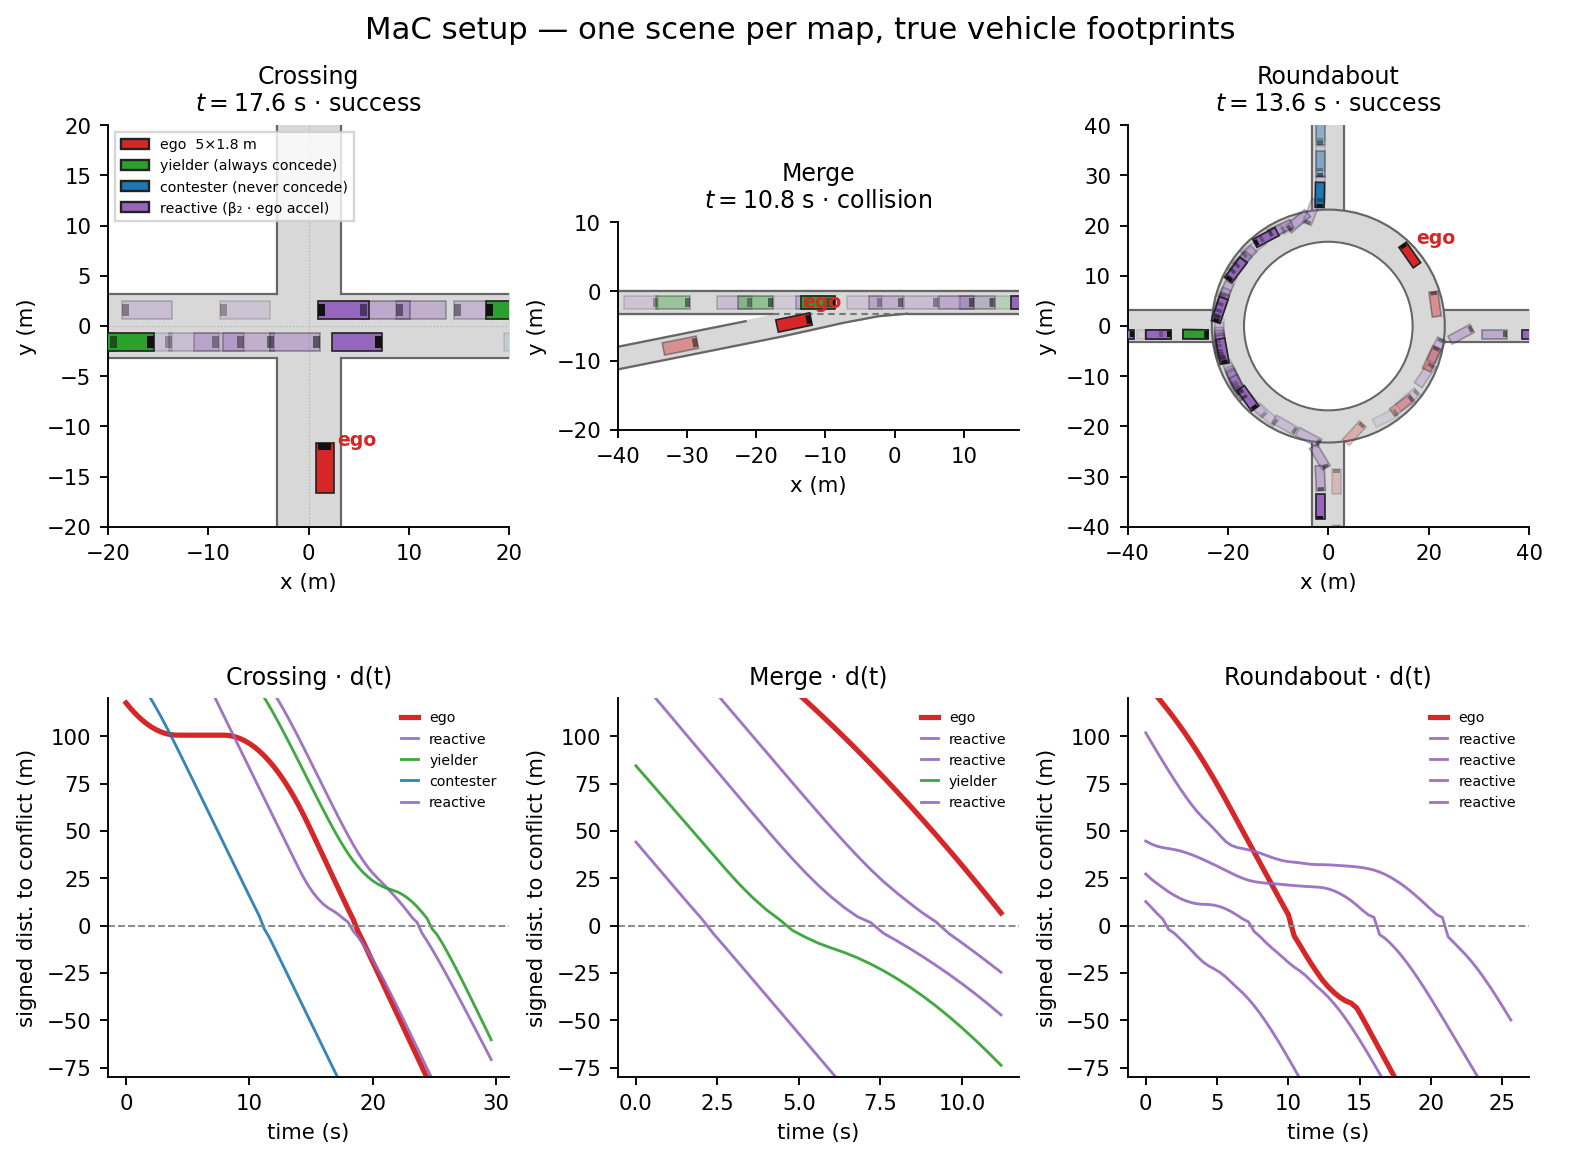
\includegraphics[width=0.75\textwidth]{figures/setup_overview.png}
\caption{Simulator setup. One snapshot per map (crossing, merge, roundabout) with $5{\times}1.8$\,m footprints.}
\label{fig:setup}
\end{figure*}

Each background vehicle is assigned a hidden type at insertion: a \emph{yielder} always concedes, a \emph{contester} never does, and a \emph{reactive} driver decides on approach. Types are drawn with probabilities $(0.1, 0.1, 0.8)$ over (yielder, contester, reactive), so most neighbours are
influenceable. For a reactive driver at signed
distance $d^i$ from the conflict point, the concession probability is
\begin{align}
\Prob(\theta^i = \yield \mid \tau^0)
&= \sigma\!\big(\beta_1 (\mathrm{TTC}^i - \mathrm{TTC}^0)
+ \beta_2\, \bar a^0 + \beta_0\big), \nonumber \\
(\beta_1,\beta_2,\beta_0) &= (0.3,\, 2.5,\, -0.3),
\label{eq:channel}
\end{align}
implemented in \texttt{SocialDriverManager.\_decide\_yield}. Here $\bar a^0$ is
a $0.8$\,s exponential moving average of the ego's \emph{commanded} acceleration
(decision interval $\Delta = 0.4$\,s), and the driver commits once it is within
$35$\,m of the conflict on the crossing and merge ($22$\,m on the roundabout,
with an incoming-edge allowlist). An unobservable per-driver offset
(``stubbornness'') is drawn at insertion and added to the logit, so the
commitment is not a deterministic function of quantities already visible in
$h$. On commit, a concession also issues an explicit \texttt{slowDown} (and a
contest holds or raises speed), so the interventional response is kinematic
inside the $F$-step prediction horizon rather than a silent junction-model
switch. The two $\beta$ terms have distinct meanings.
The first is priority: a neighbour concedes more readily when the ego will
plainly arrive first. The second is \emph{communication}: an ego that
accelerates is claiming the conflict point and raises the probability that the
other driver concedes, whereas an ego that decelerates is offering to give way
and invites the other driver to take it. Setting $\beta_2 = 0$ severs the
\emph{type}-channel while leaving geometry, type priors, and traffic density
untouched. SUMO car-following still reacts to the ego, so $\beta_2=0$ is not
``no interaction'': it is ``latent type independent of ego motion.'' That is the
control in Section~\ref{sec:exp:influence}.

The channel is known to the simulator and never exposed to the agent, which is
what lets us ask whether a learned model recovers it. We are explicit in
Section~\ref{sec:limitations} that this is a designed channel, not one estimated
from naturalistic driving.

\paragraph{Reward.} Writing $n^{\text{brake}}_t$ for the number of hard braking
events the ego \emph{causes} in others,
\begin{align}
r_t &= \underbrace{w_p \tfrac{v_t}{v_{\max}} - w_\tau}_{\text{progress}}
- \underbrace{w_c \mathbb{1}\{\text{collision}\}}_{\text{safety}} \nonumber \\
&\quad + \underbrace{w_g \mathbb{1}\{\text{arrival}\}}_{\text{goal}}
- \underbrace{w_{\text{to}} \mathbb{1}\{\text{timeout}\}}_{\text{liveness}} \nonumber \\
&\quad - \underbrace{w_a a_t^2 + w_j (\dot a_t / 10)^2}_{\text{comfort}} \nonumber \\
&\quad - \underbrace{w_x (\delta_x - g_t)^+}_{\text{proximity}}
- \underbrace{w_s\, n^{\text{brake}}_t}_{\text{social}} ,
\label{eq:reward}
\end{align}
with $(w_p, w_\tau, w_c, w_g, w_{\text{to}}, w_a, w_j, w_x, w_s) =
(0.2, 0.06, 20, 20, 15, 0.005, 0.01, 0.05, 0.15)$ and $\delta_x = 8$\,m.
The elevated time penalty ($w_\tau{=}0.06$) makes waiting for a natural gap
costly relative to the success bonus, so negotiation can pay for itself.
The jerk term is scaled by $10$ so that typical decision-to-decision accel
changes do not dominate progress. Further discussion of the social and
liveness terms is in Appendix~\ref{app:reward}.

%==============================================================================
\section{Plan-conditioned diffusion world model}
\label{sec:model}
%==============================================================================

\paragraph{Residual target.} Background traffic is close to constant velocity, so
predicting absolute motion spends capacity on the trivial component. We predict
the residual from a constant-velocity roll-out,
\begin{align}
y^i_{t,f} &= \frac{\big(p^i_{t+f} - p^i_t\big) - v^i_t\, f \Delta}{\lambda},
\quad f = 1,\dots,F, \nonumber \\
\lambda &= 8\,\text{m}.
\label{eq:residual}
\end{align}
All behaviour of interest (e.g., braking to yield, holding speed to contest)
lives in $y$.

\paragraph{Objective.} Let $c_t = \mathrm{Enc}_\phi(h_t, u_t)$ be the context and
let $m^i_f$ mask vehicles absent at step $f$. With a cosine schedule
$\bar\alpha_k$ and $y_k = \sqrt{\bar\alpha_k}\,y_0 + \sqrt{1-\bar\alpha_k}\,
\varepsilon$, the model minimises
\begin{align}
\mathcal{L}(\phi)
&= \Expect_{k,\varepsilon,(h,u,y)}\!\left[
\frac{\sum_{i,f} m^i_f \|\varepsilon - \varepsilon_\phi(y_k,k,c)\|^2}
{\sum_{i,f} m^i_f}\right] \nonumber \\
&\quad + \eta\, \Expect\big[\mathcal{H}\big(\theta^i,\, q_\phi(\cdot \mid h,u)\big)\big],
\quad \eta = 1.0,
\label{eq:loss}
\end{align}
where $q_\phi(\theta^i \mid h_t, u_t)$ is an auxiliary intention head sharing the
encoder. The default $\eta$ is $1.0$; on the crossing and roundabout the trained
models use a larger intention weight (Appendix~\ref{app:impl}). Note that $q_\phi$ estimates a \emph{plan-conditioned} belief (e.g., the
probability that neighbour $i$ concedes \emph{if the ego executes $u_t$}) which
is a counterfactual query against the channel, not a passive estimate.
Cross-entropy is restricted to open-loop (constant / hold / plan) episodes, so
the head is fitted to $p(\theta \mid h, \mathrm{do}(u))$ rather than the
observational conditional in which $u$ is a function of $h$. Training also
drops the plan with probability $0.1$, which gives the encoder a well-defined
history-only branch.

The essential structural choice is that $c_t$ depends on $u_t$. The model is
therefore controllable, $p_\phi(y \mid h, u)$, and can be queried
counterfactually. Sampling uses a strided DDIM schedule with $x_0$ clipping,
which keeps a query cheap enough to run inside the RL loop. At query time the
intention logits are written as a history-only term plus a plan residual, and
the residual is scaled by a guidance weight $w$ calibrated on held-out open-loop
cross-entropy and stored in the checkpoint ($w{=}1$ is the plain conditional).

\paragraph{Identification: why the counterfactual query is licensed.}

Identification is achieved through exogenous action variation in the data collection policy; details are provided in Appendix~\ref{app:identification}.

%==============================================================================
\section{Negotiation-aware planning}
\label{sec:planning}
%==============================================================================

\paragraph{Belief features.} The closed-loop policy uses \texttt{plan\_action}:
the discrete action is itself a probe from
$\mathcal{U}=\{-4,0,+3\}$ (yield / hold / assert), held for
$\texttt{commit\_steps}=10$ environment steps ($4$\,s), shorter than the
$F{=}20$ query horizon so the policy can still wait out a hard contester. For each $u \in \mathcal{U}$ the encoder draws
$S$ futures $y^{(1:S)} \sim p_\phi(\cdot \mid h_t, u)$ with deterministic DDIM
($\eta{=}0$) and a shared latent across the probe batch so differences isolate
$u$, and forms
\begin{equation}
g_s(u) = \min_{f,i} \big\| p^0_f(u) - \hat p^{i,(s)}_f \big\|,
\label{eq:clearance}
\end{equation}
the closest approach between the probe ego trajectory and predicted neighbours
(the $K$ nearest within a radius, not an oracle of who is about to commit).
Risk, margin and spread of $g_s(u)$ can be produced by ego geometry alone when a
constant-velocity neighbour forecast already moves them when the probe
accelerates so they do not identify negotiation. Learned arms therefore
reuse the same deterministic CV core stats for risk/clearance and add residual
features the CV baseline cannot copy. The encoder also writes, for each $u$,
(i)~the predicted closest-neighbour position at mid- and end-horizon and
(ii)~the mean displacement of predicted neighbours relative to the hold probe,
\begin{equation}
\Delta(u)=\frac{1}{|\mathcal{N}|}\sum_{i\in\mathcal{N}}
\big\| \bar p^{i}(u) - \bar p^{i}(0) \big\|,
\label{eq:delta}
\end{equation}
which is identically zero unless the forecast of $y$ itself moves with $u$. A \texttt{geometry} or \texttt{history} encoder has $\Delta\equiv 0$; only a plan-conditioned model can make it nonzero. Details are in Appendix~\ref{app:Belief}.

The policy $\pi_\vartheta(a_t \mid o_t, \psi_t)$ maximises
$J(\vartheta) = \Expect_{\pi_\vartheta}[\sum_t \gamma^t r_t]$ with
$\theta^i \sim \rho(\cdot \mid \tau^0)$, using clipped PPO
\cite{schulman2017proximal} with a running observation normalisation: raw
kinematics and belief features differ by two orders of magnitude, and without
per-feature scaling a small-magnitude slot such as $\Delta(u)$ is effectively
absent from a tanh trunk. In the simulator $J$ is a negotiation objective.
Probe risk can still support ordinary risk-aware planning, which a history-only
or geometry encoder already provides. What those encoders \emph{cannot} provide
is a nonzero $\Delta(u)$. A closed-loop diffusion--geometry gap under this
interface cannot be explained as ``the policy only saw a collision margin'';
the absence of such a gap cannot be blamed on that bottleneck either.
Section~\ref{sec:exp:planner}--\ref{sec:exp:influence} report which of those
two readings the data support.

%==============================================================================
\section{What can be proved}
\label{sec:theory}
%==============================================================================

The following results characterize the theoretical properties of the proposed formulation.
We show that point-forecast planning can be suboptimal in the considered setting and bound the influence contribution by the sensitivity of the channel.

\begin{proposition}[Certainty-equivalence regret]
\label{prop:ce}
Consider one decision with binary latent $\theta \in \{Y, C\}$, $\Prob(\theta =
Y) = p$, and actions $\{\textit{go}, \textit{wait}\}$ with $c(\textit{go}, Y) =
0$, $c(\textit{go}, C) = C > 0$, $c(\textit{wait}, \cdot) = d > 0$. A
distributional planner attains $\min\{(1-p)C, d\}$. A certainty-equivalence
planner that replaces $\theta$ by its most likely value and acts optimally for it
chooses \textit{go} whenever $p > 1/2$, incurring true expected cost $(1-p)C$.
Its regret is $\mathcal{R} = \max\{0, (1-p)C - d\}$, strictly positive whenever
$d < (1-p)C$.
\end{proposition}
\begin{proof}
Immediate by comparing the two expected costs.
\end{proof}

The regime $d < (1-p)C$ is precisely an unprotected crossing: waiting is cheap,
collisions are expensive, and residual contest probability is far from zero.
Proposition~\ref{prop:ce} also explains why a \emph{mean-trajectory} forecast is
worse than a mode: averaging a yielding and a contesting trajectory produces a
path no driver would execute, so the planner optimises against a future of
probability zero. We stress that the
proposition is a statement about certainty equivalence in a one-shot decision; it
explains why the failure mode exists, and does not bound the RL agent's regret.

The next result is the one that carries weight, because it makes the value of
negotiation measurable rather than rhetorical.

\begin{proposition}[Negotiation gain is bounded by channel sensitivity]
\label{prop:influence}
Let $R(u,\theta) \in [0, R_{\max}]$ and $J(u) = \Expect_{\theta \sim \rho(\cdot
\mid u)}[R(u,\theta)]$. For any plans $u, u_0$, decompose
\begin{align}
J(u) - J(u_0)
&= \underbrace{\Expect_{\theta \sim \rho(\cdot \mid u_0)}\big[R(u,\theta) - R(u_0,\theta)\big]}_{G_{\mathrm{plan}}} \nonumber \\
&\quad + \underbrace{\Expect_{\theta \sim \rho(\cdot \mid u)}[R(u,\theta)]
- \Expect_{\theta \sim \rho(\cdot \mid u_0)}[R(u,\theta)]}_{G_{\mathrm{infl}}} .
\end{align}
Then the influence term obeys
\begin{equation}
\big|G_{\mathrm{infl}}\big| \;\le\; R_{\max}\cdot \TV\!\big(\rho(\cdot \mid u),\, \rho(\cdot \mid u_0)\big),
\label{eq:tvbound}
\end{equation}
and $G_{\mathrm{infl}} = 0$ for every $u$ whenever $\rho$ does not depend on $u$.
For binary $\Theta$ the bound is
$|G_{\mathrm{infl}}| \le R_{\max}\,|\Prob(\yield \mid u) - \Prob(\yield \mid u_0)|$.
\end{proposition}
\begin{proof}
The decomposition is an addition and subtraction of
$\Expect_{\rho(\cdot \mid u_0)}[R(u,\theta)]$. For the bound, $G_{\mathrm{infl}}
= \int R(u,\theta)\,\big(\rho(d\theta \mid u) - \rho(d\theta \mid u_0)\big)$, and
for any $f$ with range in an interval of length $L$,
$|\int f\,d(P - Q)| \le L\cdot\TV(P,Q)$; take $L = R_{\max}$. If $\rho(\cdot \mid
u) = \rho(\cdot \mid u_0)$ the integrand measure is zero.
\end{proof}

Proposition~\ref{prop:influence} is the formal content of ``motion is
communication'', and unlike a feasibility argument it says something with
consequences. The gain attributable to influence is \emph{at most} the reward
scale times how far the ego can move the type distribution, so an environment
with a weak channel cannot reward negotiation however good the model is. It also
yields a falsifiable prediction: setting $\beta_2 = 0$ in
Eq.~\eqref{eq:channel} forces $\TV = 0$, hence $G_{\mathrm{infl}} = 0$, and any
advantage of a plan-conditioned model over a history-only one must disappear.
Section~\ref{sec:exp:influence} tests this. In our simulator the kernel is known,
so the bound can be evaluated: at zero priority margin the probe set spans
$\Prob(\yield)$ from \probeYieldBrake{} to \probeYieldAssert{} under the true
kernel, giving $\TV = \gtTV$.

\begin{remark}[Resolution of the sampled risk estimate]
\label{rem:hoeffding}
$\hat P_S(u) = \frac{1}{S}\sum_s \mathbb{1}\{g_s(u) < \delta\}$ is unbiased for
the conflict probability under $p_\phi$, and by Hoeffding
$\Prob(|\hat P_S - P| \ge \epsilon) \le 2\exp(-2S\epsilon^2)$. At $S = 8$ the
$95\%$ resolution is only $\epsilon \approx 0.48$, so a single-step risk estimate
is coarse; the policy sees a temporal sequence of such estimates, which mitigates
this. Because $S$ is therefore a first-order design parameter rather than an
incidental hyperparameter, we sweep it in Section~\ref{sec:exp:sweep}.
\end{remark}

%==============================================================================
\section{Experiments}
\label{sec:exp}
%==============================================================================

We test three claims separately, because a single closed-loop number cannot
tell them apart.

\begin{enumerate}\itemsep2pt
\item[\textbf{Q1}] \textbf{Prediction.} Can $p_\phi(y\mid h,u)$ forecast
neighbours, and how does it compare to constant velocity and to $p(y\mid h)$
(\S\ref{sec:exp:wm})?
\item[\textbf{Q2}] \textbf{Counterfactual prediction.} Given the same $h$, does
changing $u$ move the forecast in the direction of the simulator's
$\mathrm{do}(u)$ response (\S\ref{sec:exp:channel})?
\item[\textbf{Q3}] \textbf{Useful negotiation.} Does giving those queries to an
RL planner improve decisions beyond a history-only world model, and does that
extra gain vanish when the type-channel is off
(\S\ref{sec:exp:planner}--\ref{sec:exp:influence})?
\end{enumerate}

\paragraph{Protocol.} The operating point matches the released pipeline: channel
Eq.~\eqref{eq:channel} with $(\beta_1,\beta_2,\beta_0)=(0.3,2.5,-0.3)$ and
type mix $(0.1,0.1,0.8)$ on the merge and roundabout; the crossing closed-loop
suite uses a louder channel $(\beta_1,\beta_2)=(0.15,4.0)$ and type mix
$(0.15,0.15,0.7)$ so negotiation is not saturated by natural gaps. Decision
distance $35$\,m on the crossing and merge ($22$\,m on the roundabout), intent
window $0.8$\,s, prediction horizon $F{=}20$ ($8$\,s), probes $\{-4,0,+3\}$,
and five belief arms (\texttt{none}, \texttt{geometry}, \texttt{kernel},
\texttt{history}, \texttt{diffusion}) on each of the three scenes, up to $10$
seeds, $60$ PPO iterations, with \texttt{plan\_action} and
$\texttt{commit\_steps}{=}10$ ($4$\,s).
\numEpisodes{} crossing episodes (plus merge/roundabout, collected the same way)
yield \numTrainSamples{} training and \numValSamples{} validation samples on
the crossing. The split is over paired-intervention groups / episodes,
not individual overlapping samples. Consecutive decision steps within an
episode produce near-identical windows, so a random sample split would inflate
validation metrics.

\subsection{Q1: Prediction}
\label{sec:exp:wm}

Table~\ref{tab:worldmodel} reports displacement errors. The comparison protocol
matters more than the numbers. minFDE is a best-of-$S$ statistic and it is not
meaningful to compare it against a single deterministic forecast: doing so
credits the generative model for sample diversity without charging it for
calibration. We therefore report a constant-velocity roll-out perturbed by
Gaussian noise at the empirical residual scale (\residStd{}\,m) with the same
$S=8$ budget, alongside the deterministic roll-out, and we report meanFDE as well
as minFDE. Against that protocol minFDE is a win --- \wmMinFDE{}\,m versus
\cvsMinFDE{}\,m for the matched stochastic baseline. The same comparison on all three maps is in Appendix~\ref{app:impl} (Fig.~\ref{fig:wm-fde}). MeanFDE
(\wmMeanFDE{}\,m) exceeds deterministic constant velocity (\cvMeanFDE{}\,m)
on the crossing, as expected when a multi-hypothesis model spreads mass over
modes that a single CV roll-out never visits.
Plan-conditioning on the \emph{logged} $u$ is a weak test of Q2: if zeroing $u$
at eval time barely changes FDE, $u$ was not needed to predict the realised
future. We report that ablation in Table~\ref{tab:worldmodel}
(\wmZeroMinFDE{}\,m with the plan zeroed vs \wmMinFDE{}\,m with the plan;
history-only \histMinFDE{}\,m).

\begin{table*}[!t]
\caption{Displacement error on held-out crossing episodes, in metres, $K=5$ neighbours over $F=20$ steps ($8$\,s). minFDE is a best-of-$S$ statistic and is only comparable across rows with the same $S$; the deterministic constant-velocity roll-out is the reference for meanFDE, and the noise-perturbed roll-out with a matched $S=8$ budget is the reference for minFDE.}
\label{tab:worldmodel}
\centering
\begin{tabular}{|l|c|c|c|c|c|}
\hline
\textbf{Model} & $\boldsymbol{S}$ & \textbf{minFDE} & \textbf{meanFDE} & \textbf{minADE} & \textbf{meanADE} \\
\hline
Constant velocity & 1 & \cvMinFDE{} & \cvMeanFDE{} & \cvMinADE{} & \cvMeanADE{} \\
\hline
Constant velocity $+$ noise & 8 & \cvsMinFDE{} & \cvsMeanFDE{} & \cvsMinADE{} & \cvsMeanADE{} \\
\hline
Diffusion $p(y\mid h,u)$ (DDIM $T{=}\wmT{}$) & 8 & \wmMinFDE{} & \wmMeanFDE{} & \wmMinADE{} & \wmMeanADE{} \\
\hline
Diffusion $p(y\mid h)$ (plan zeroed) & 8 & \wmZeroMinFDE{} & \wmZeroMeanFDE{} & \wmZeroMinADE{} & \wmZeroMeanADE{} \\
\hline
History-only WM $p(y\mid h)$ & 8 & \histMinFDE{} & \histMeanFDE{} & \histMinADE{} & \histMeanADE{} \\
\hline
\end{tabular}
\end{table*}

\subsection{Q2: Counterfactual prediction}
\label{sec:exp:channel}

Q2 is not ``FDE on logged $(h,u,y)$.'' It is: same $h$, different $u$, different
$y$. Table~\ref{tab:channel} and Fig.~\ref{fig:channel} probe the intention head on the crossing; Fig.~\ref{fig:channel-scenes} in Appendix~\ref{app:impl} repeats the probe on all three maps. A model that had memorised the marginal would show no probe dependence, and one that had learned a spurious correlate could show the reverse. Trajectory shift is reported against sample spread: a probe effect smaller than the model's own noise is not usable. An interventional replay of the same scene under $\mathrm{do}(u)$
(Appendix~\ref{app:impl}, Table~\ref{tab:cf} and Fig.~\ref{fig:cf-shift})
scores forecasts against realised neighbour futures; a history-only model must predict nearly the same $y$ for every $u$.

\begin{table*}[!t]
\caption{Channel recovery on the crossing. The model is probed with
$\{-4,0,+3\}$; the simulator's kernel requires $\Pr(\yield)$ to increase with
ego acceleration. Trajectory shift is the mean displacement of the predicted
futures relative to the hold probe, to be read against the spread across
diffusion samples (\probeSpread{}\,m). Ground truth uses the held-out scene's
TTC margin (scene-conditioned).}
\label{tab:channel}
\centering
\begin{tabular}{|l|c|c|c|c|c|}
\hline
\textbf{Probe} $\boldsymbol{u}$ & $\boldsymbol{a}$ \textbf{(m/s}$^{\boldsymbol{2}}$\textbf{)} & \textbf{$\Pr(\yield)$ dec.} & \textbf{$\Pr(\yield)$ all} & \textbf{$\Pr(\yield)$ truth} & \textbf{Shift (m)} \\
\hline
\textit{yield} & $-4$ & \probeModelBrake{} & \probeModelAllBrake{} & \probeYieldBrake{} & \probeShiftBrake{} \\
\hline
\textit{hold} & $0$ & \probeModelHold{} & \probeModelAllHold{} & \probeYieldHold{} & --- \\
\hline
\textit{assert} & $\assertAccel{}$ & \probeModelAssert{} & \probeModelAllAssert{} & \probeYieldAssert{} & \probeShiftAssert{} \\
\hline
Total variation & & \tvModelDec{} & \tvModelAll{} & \gtTV{} & \\
\hline
Monotone in $a$ & & yes & yes & yes & \\
\hline
\end{tabular}
\end{table*}

\begin{figure*}[!t]
\centering
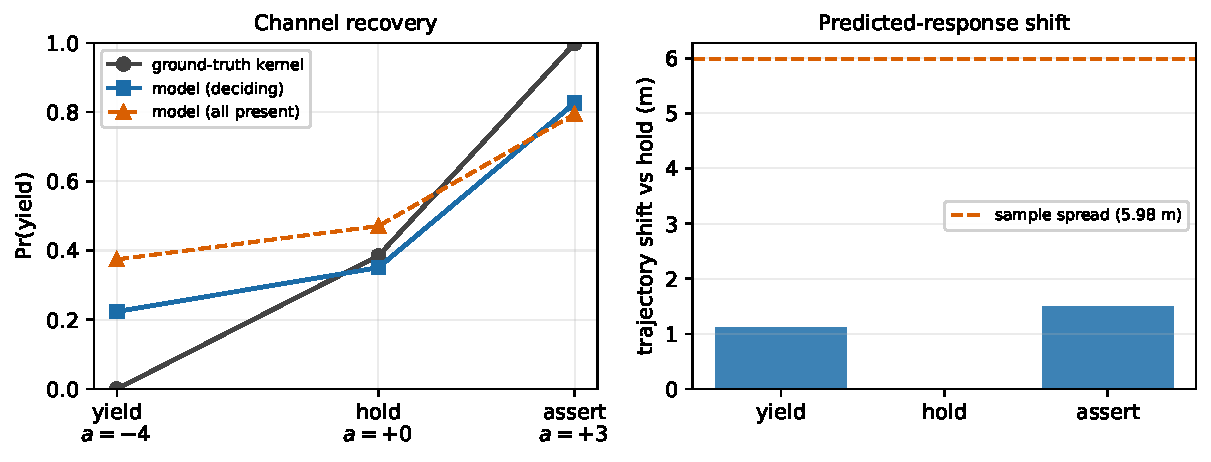
\includegraphics[width=0.8\textwidth]{figures/channel.pdf}
\caption{Left: probe response of the learned intention head against the
simulator's influence kernel. Right: mean trajectory shift of predicted
futures relative to the hold probe, compared to the model's own sample
spread (dashed).}
\label{fig:channel}
\end{figure*}

Probe TV collapses if averaged over all neighbours; we report the deciding
population (Appendix~\ref{app:impl}). Even there, recovered TV is weaker than
the kernel and trajectory shifts sit near sample spread.

\subsection{Q3: Useful negotiation}
\label{sec:exp:planner}

Q3 asks whether counterfactual queries improve \emph{decisions} beyond
$p(y\mid h)+$RL. A fair test has to survive a specific objection: the policy
never sees the sample tensor, only a summary, and a summary built from
$g_s(u)$~\eqref{eq:clearance} can be reproduced by ego geometry alone. The
encoder of Section~\ref{sec:planning} answers that objection by adding waypoints
and $\Delta(u)$~\eqref{eq:delta}. Geometry and history then have
$\Delta\equiv 0$; a remaining diffusion--geometry gap cannot be ``the policy
only saw a smaller collision margin,'' and a remaining tie cannot be blamed on
that bottleneck either. The \texttt{kernel} arm is the engineered channel
baseline: coefficients of the same logistic form as Eq.~\eqref{eq:channel} are
fitted offline by logistic regression on the world-model dataset (priority
margin and an EMA of plan acceleration), then frozen for planning---not read
from the live simulator. A diffusion--geometry gap that \texttt{kernel} also
matches is consistent with influence; a gap that history also matches is not.

Table~\ref{tab:planner} reports the crossing; Table~\ref{tab:merge} the merge;
Table~\ref{tab:roundabout} the roundabout; Figs.~\ref{fig:planner-return} and \ref{fig:paired-delta} summarize the same numbers. In the Appendix, Fig.~\ref{fig:curves} shows the crossing learning curves, and Fig.~\ref{fig:curves-scenes} shows all three maps.

The comparison that matters is
\texttt{none} versus \texttt{geometry} versus \texttt{kernel} versus
\texttt{history} versus \texttt{diffusion}. A large
\texttt{none}$\to$\texttt{geometry} lift with
\texttt{history}$\approx$\texttt{diffusion} is risk-aware planning, not
negotiation. A remaining diffusion--history \emph{and} diffusion--geometry gap
on return, with paired bootstrap CIs excluding zero, is the evidence Q3
requires.

On the \textbf{merge}, diffusion returns \MergeDiffusionReturn{} versus
geometry \MergeGeometryReturn{} and history \MergeHistoryReturn{}
(paired $\Delta$ return vs geometry \MergediffusionRet{}, $95\%$ CI
$[\MergediffusionRetLo{},\MergediffusionRetHi{}]$, $n{=}\MergediffusionRetN{}$).
History does not significantly beat geometry. These
results suggest that the gain is related to plan conditioning rather than
simply the use of a learned world model.

On the \textbf{crossing}, under a stronger influence channel
($\beta_2{=}4.0$, $\beta_1{=}0.15$, type mix $0.15/0.15/0.7$), diffusion
returns \DiffusionReturn{} versus geometry \GeometryReturn{} (paired
$\Delta$ return \diffusionRet{}, $95\%$ CI
$[\diffusionRetLo{},\diffusionRetHi{}]$, $n{=}\diffusionRetN{}$). The CI
excludes zero, as do the paired success and collision intervals. History
(\HistoryReturn{}) and the offline-fitted kernel (\KernelReturn{}) sit between
\texttt{none} and diffusion and do not significantly beat geometry; the
diffusion--geometry gap is therefore the plan-conditioned neighbour forecast,
not risk geometry alone.

On the \textbf{roundabout}, after rebalancing background demand so the ego's
entry lane and exit ring stay clear, diffusion returns \RaDiffusionReturn{}
versus geometry \RaGeometryReturn{} (paired $\Delta$ return \RadiffusionRet{},
$95\%$ CI $[\RadiffusionRetLo{},\RadiffusionRetHi{}]$,
$n{=}\RadiffusionRetN{}$). Diffusion ranks first on mean return and success,
but the CI still includes zero. Kernel (\RaKernelReturn{}) and history
(\RaHistoryReturn{}) no longer beat geometry; the scene remains harder to
separate than the merge or the strengthened crossing.

\begin{table*}[!t]
\caption{Closed-loop performance on the crossing (commit\_steps$=10$, plan-as-action, $F=20$), mean $\pm$ s.d.\ over $n{=}10$ seeds.}
\label{tab:planner}
\centering
\begin{tabular}{|l|c|c|c|c|c|c|}
\hline
\textbf{Belief} & \textbf{Success (\%)} & \textbf{Collision (\%)} & \textbf{Timeout (\%)} & \textbf{Return} & \textbf{Crossing steps} & \textbf{Induced brakes} \\
\hline
\texttt{none} (no world model) & 61.60$\pm$4.45 & 38.40$\pm$4.45 & 0.00$\pm$0.00 & 8.55$\pm$1.73 & 59.22$\pm$1.72 & 0.00$\pm$0.00 \\ % n=10
\texttt{geometry} (ego-plan CV risk) & 63.60$\pm$3.67 & 36.20$\pm$4.14 & 0.20$\pm$0.60 & 9.21$\pm$1.23 & 60.22$\pm$2.20 & 0.00$\pm$0.00 \\ % n=10
\texttt{kernel} (analytic channel feature) & 64.80$\pm$3.25 & 34.60$\pm$3.80 & 0.60$\pm$1.28 & 9.65$\pm$1.25 & 60.02$\pm$3.18 & 0.00$\pm$0.00 \\ % n=10
\texttt{history} (plan dropped) & 65.60$\pm$3.20 & 34.40$\pm$3.20 & 0.00$\pm$0.00 & 9.95$\pm$1.09 & 60.74$\pm$3.19 & 0.00$\pm$0.00 \\ % n=10
\texttt{diffusion} (plan-conditioned) & 68.00$\pm$3.10 & 31.80$\pm$3.40 & 0.20$\pm$0.60 & 10.82$\pm$1.11 & 62.98$\pm$5.20 & 0.00$\pm$0.00 \\ % n=10
\hline
\end{tabular}
\end{table*}

\begin{figure}[!t]
\centering
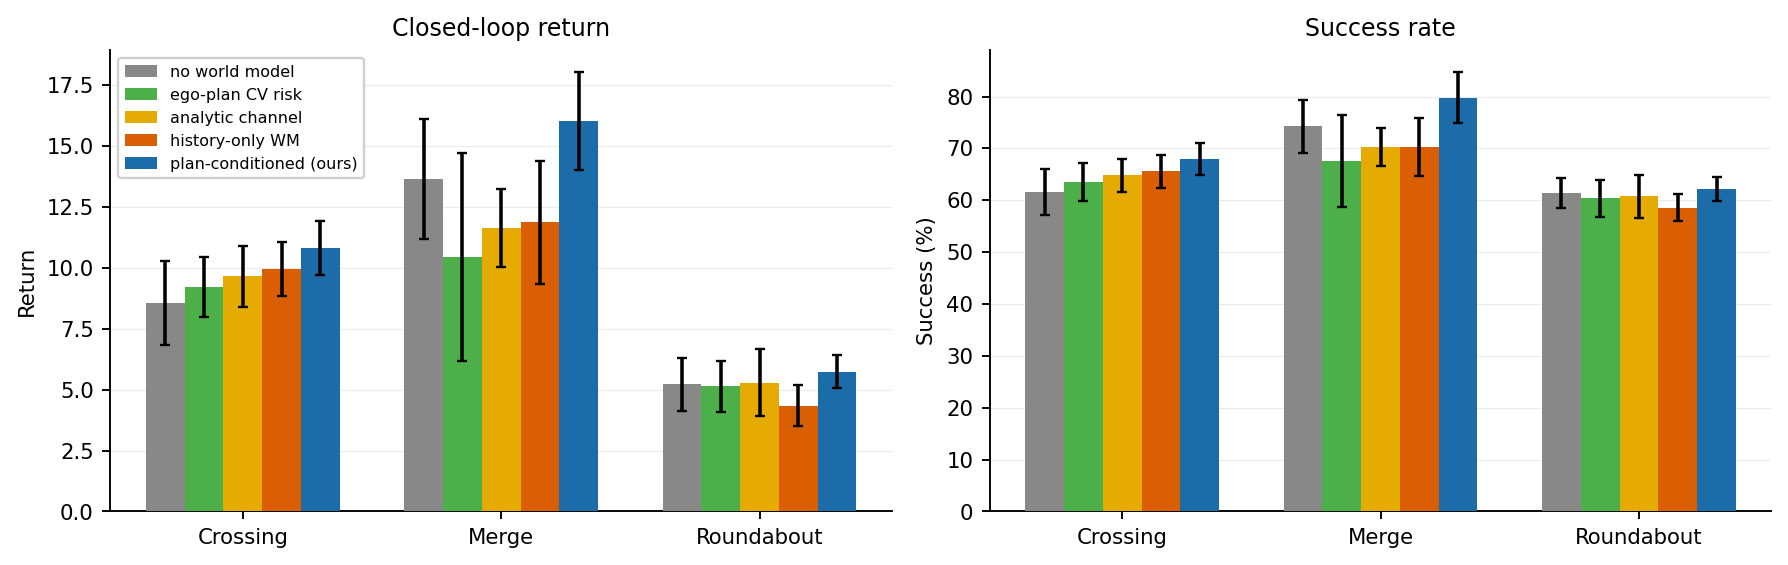
\includegraphics[width=0.4\textwidth]{figures/results_extra/planner_returnv2.png}
\caption{Closed-loop return and success on all three maps (mean $\pm$ s.d.\ over
seeds). Plan-conditioned diffusion leads on the merge and the crossing; on the
roundabout the arms stay closer together.}
\label{fig:planner-return}
\end{figure}

\begin{figure*}[!t]
\centering
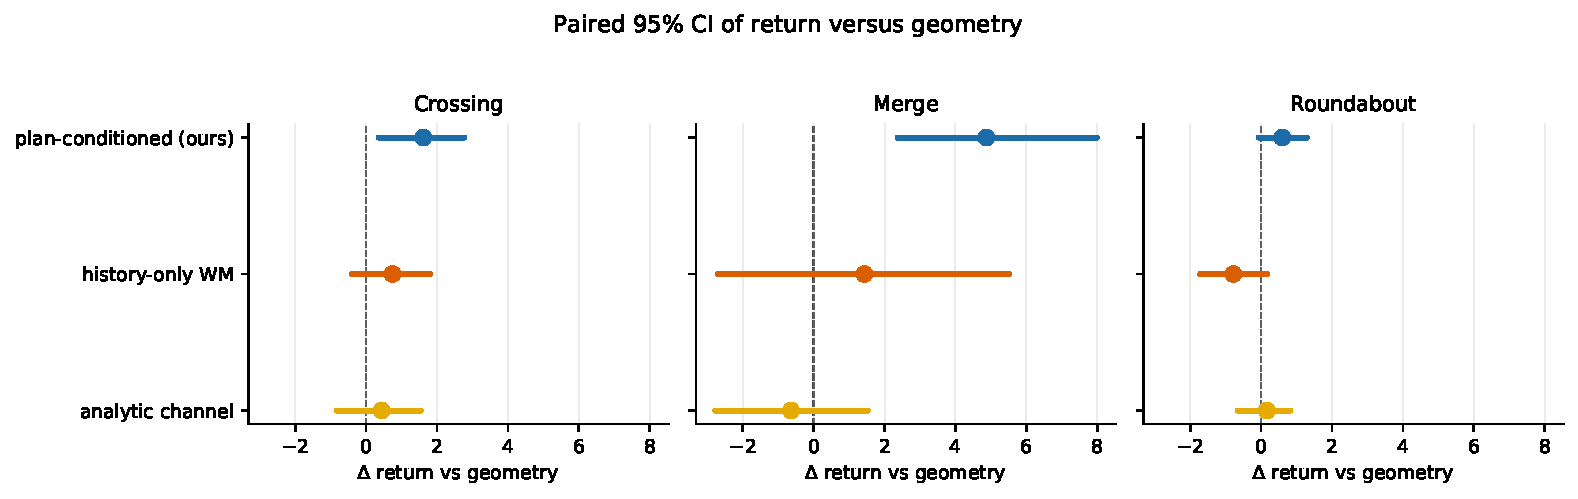
\includegraphics[width=0.96\textwidth]{figures/results_extra/paired_delta.pdf}
\caption{Paired $95\%$ CI of return versus the geometry arm, seed-matched.
The CI excludes zero for diffusion on the merge and the crossing. Roundabout
CIs all include zero.}
\label{fig:paired-delta}
\end{figure*}

\begin{table*}[!t]
\caption{Closed-loop performance on the merge (commit\_steps$=10$, plan-as-action, $F=20$), mean $\pm$ s.d.\ over seeds.}
\label{tab:merge}
\centering
\begin{tabular}{|l|c|c|c|c|c|c|}
\hline
\textbf{Belief} & \textbf{Success (\%)} & \textbf{Collision (\%)} & \textbf{Timeout (\%)} & \textbf{Return} & \textbf{Crossing steps} & \textbf{Induced brakes} \\
\hline
\texttt{none} (no world model) & 74.25$\pm$5.04 & 25.25$\pm$3.86 & 0.50$\pm$1.32 & 13.64$\pm$2.45 & 76.35$\pm$1.16 & 0.00$\pm$0.00 \\ % n=8
\texttt{geometry} (ego-plan CV risk) & 67.56$\pm$8.83 & 30.67$\pm$6.11 & 1.78$\pm$3.33 & 10.43$\pm$4.28 & 77.55$\pm$1.42 & 0.00$\pm$0.00 \\ % n=9
\texttt{kernel} (analytic channel feature) & 70.29$\pm$3.61 & 28.57$\pm$3.16 & 1.14$\pm$0.99 & 11.64$\pm$1.60 & 77.41$\pm$1.73 & 0.00$\pm$0.00 \\ % n=7
\texttt{history} (plan dropped) & 70.22$\pm$5.61 & 29.78$\pm$5.61 & 0.00$\pm$0.00 & 11.87$\pm$2.52 & 77.40$\pm$0.50 & 0.00$\pm$0.00 \\ % n=9
\texttt{diffusion} (plan-conditioned) & 79.78$\pm$4.94 & 20.00$\pm$5.08 & 0.22$\pm$0.63 & 16.02$\pm$2.01 & 79.23$\pm$1.36 & 0.00$\pm$0.00 \\ % n=9
\hline
\end{tabular}
\end{table*}

\begin{table*}[!t]
\caption{Closed-loop performance on the roundabout (commit\_steps$=10$, plan-as-action, $F=20$), mean $\pm$ s.d.\ over $n{=}10$ seeds.}
\label{tab:roundabout}
\centering
\begin{tabular}{|l|c|c|c|c|c|c|}
\hline
\textbf{Belief} & \textbf{Success (\%)} & \textbf{Collision (\%)} & \textbf{Timeout (\%)} & \textbf{Return} & \textbf{Crossing steps} & \textbf{Induced brakes} \\
\hline
\texttt{none} (no world model) & 61.40$\pm$2.84 & 38.60$\pm$2.84 & 0.00$\pm$0.00 & 5.21$\pm$1.09 & 87.60$\pm$2.41 & 0.00$\pm$0.00 \\ % n=10
\texttt{geometry} (ego-plan CV risk) & 60.40$\pm$3.56 & 39.60$\pm$3.56 & 0.00$\pm$0.00 & 5.13$\pm$1.04 & 85.47$\pm$2.67 & 0.00$\pm$0.00 \\ % n=10
\texttt{kernel} (analytic channel feature) & 60.80$\pm$4.12 & 39.20$\pm$4.12 & 0.00$\pm$0.00 & 5.29$\pm$1.39 & 85.00$\pm$3.85 & 0.00$\pm$0.00 \\ % n=10
\texttt{history} (plan dropped) & 58.60$\pm$2.54 & 41.40$\pm$2.54 & 0.00$\pm$0.00 & 4.34$\pm$0.85 & 85.41$\pm$2.17 & 0.00$\pm$0.00 \\ % n=10
\texttt{diffusion} (plan-conditioned) & 62.20$\pm$2.27 & 37.80$\pm$2.27 & 0.00$\pm$0.00 & 5.72$\pm$0.68 & 86.59$\pm$1.98 & 0.00$\pm$0.00 \\ % n=10
\hline
\end{tabular}
\end{table*}


\subsection{Severing the channel}
\label{sec:exp:influence}

Proposition~\ref{prop:influence} predicts that with $\beta_2 = 0$ the
type-influence term is identically zero. SUMO car-following still reacts, so a
residual gap of any world model over \texttt{none} is ordinary prediction
(including kinematic interaction) and is expected. What the proposition forbids
is an \emph{additional} gain of $p(y\mid h,u)$ over $p(y\mid h)$.
Table~\ref{tab:influence} is the matched $\beta_2=0$ control on the crossing
(Fig.~\ref{fig:beta-onoff}), run under the same type mix and margins as the
louder operating point with only $\beta_2$ set to zero ($n{=}5$ seeds).
The merge diffusion--history gap under $\beta_2>0$, together with the
significant diffusion--geometry gap on the strengthened crossing, is the
primary Q3 evidence; we did not re-run the merge suite at $\beta_2=0$.

\begin{table*}[!t]
\caption{Type-channel off ($\beta_2 = 0$). Latent types no longer depend on ego motion, so Proposition~\ref{prop:influence} forces $G_{\mathrm{infl}} = 0$. SUMO car-following still reacts to the ego. Mean $\pm$ s.d.\ over $n{=}5$ seeds.}
\label{tab:influence}
\centering
\begin{tabular}{|l|c|c|c|c|c|c|}
\hline
\textbf{Belief} & \textbf{Success (\%)} & \textbf{Collision (\%)} & \textbf{Timeout (\%)} & \textbf{Return} & \textbf{Crossing steps} & \textbf{Induced brakes} \\
\hline
\texttt{none} (no world model) & 62.00$\pm$0.00 & 38.00$\pm$0.00 & 0.00$\pm$0.00 & 9.24$\pm$0.07 & 51.03$\pm$0.19 & 0.00$\pm$0.00 \\ % n=5
\hline
\texttt{history} (plan dropped) & 64.40$\pm$2.94 & 35.60$\pm$2.94 & 0.00$\pm$0.00 & 10.00$\pm$1.12 & 52.29$\pm$0.52 & 0.00$\pm$0.00 \\ % n=5
\hline
\texttt{diffusion} (multi-hypothesis) & 64.80$\pm$2.04 & 35.20$\pm$2.04 & 0.00$\pm$0.00 & 10.25$\pm$0.94 & 52.82$\pm$1.12 & 0.00$\pm$0.00 \\ % n=5
\hline
\end{tabular}
\end{table*}

\begin{figure}[!t]
\centering
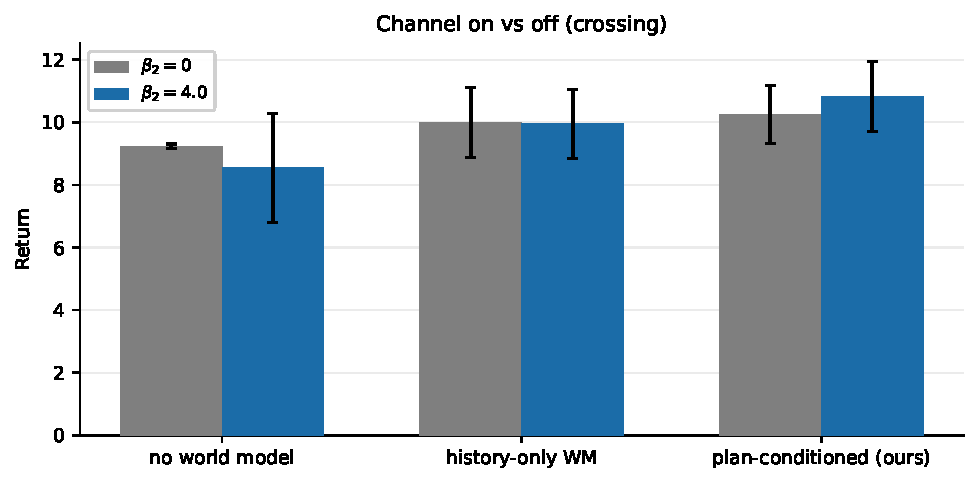
\includegraphics[width=\columnwidth]{figures/results_extra/beta_onoff.pdf}
\caption{Crossing return with the type-channel off ($\beta_2{=}0$) versus the
operating point ($\beta_2{=}4.0$). At $\beta_2{=}0$ the three arms stay close;
with the channel on, diffusion pulls ahead of \texttt{none}.}
\label{fig:beta-onoff}
\end{figure}

\subsection{Sample budget}
\label{sec:exp:sweep}

Remark~\ref{rem:hoeffding} bounds the Monte-Carlo error of the \emph{risk
feature}, not PPO sample efficiency. Table~\ref{tab:sweep} and
Fig.~\ref{fig:sweep} vary $S \in \{1, 4, 8, 16\}$. $S{=}8$ is the operating
point used elsewhere.

%==============================================================================
\section{Limitations}
\label{sec:limitations}
%==============================================================================

We state these plainly because several bear directly on how the results should
be read.

\begin{itemize}\itemsep1pt
\item \textbf{Designed channel, favourable causal structure.} $\rho$ is
synthetic. Recovery and closed-loop gains do not show that the method discovers
unknown negotiation in real traffic. $\beta_2=0$ still leaves SUMO
car-following. Recovered model TV is much weaker than the designed kernel on
the crossing and roundabout; on the merge it matches (\MergetvModelDec{} vs
\MergegtTV{}).

\item \textbf{Closed-loop gains are scene-dependent.}
On the merge and the strengthened crossing, diffusion significantly beats
\texttt{geometry}; history and the offline-fitted \texttt{kernel} do not.
On the roundabout, diffusion leads on means but the paired CI still includes
zero, and neither kernel nor history beats geometry. Influence is identifiable
on all three maps when scored on interventional probe plans; converting that
into a closed-loop gap is easiest on the merge, achievable on the crossing
under a louder channel, and still unresolved on the roundabout.

\item \textbf{Weak counterfactual trajectory signal.} Probe intention can be
directionally correct while trajectory shifts sit near sample spread.
Table~\ref{tab:cf} reports interventional FDE on $n{=}33$ matched crossing
scenes: history has lower FDE with zero shift; diffusion moves with $u$. We do
not claim a numerical CF FDE win. On the closed-loop belief interface we
therefore keep risk, clearance, and intent blocks and drop $\Delta(u)$ when
its signal-to-noise ratio is below one.

\item \textbf{Multimodality is regime-dependent.} Sample budget $S{=}8$ is the
operating point used throughout; we do not claim diffusion is universally
better at $S{=}1$.

\item \textbf{Coarse queries and a compact summary.} Three probes, $K$
nearest neighbours, no oracle of who is deciding. The policy sees a
$38$-scalar summary that includes neighbour waypoints and the influence
feature $\Delta(u)$, not the raw sample tensor. Identifying relevant
vehicles in deployment is itself hard.

\item \textbf{Limited shift and scenarios.} Results are in-family on three
SUMO maps (crossing, merge, roundabout). No published predictor/negotiator
baseline.

\item \textbf{Theory scope.} Proposition~\ref{prop:ce} is one-shot.
Proposition~\ref{prop:influence} is an upper bound. The Hoeffding result characterizes the finite-sample resolution of the risk estimator and should not be interpreted as a bound on PPO sample efficiency.
\end{itemize}

%==============================================================================
\section{Conclusion}
%==============================================================================

We formalised negotiation at unprotected conflict points as an influence channel
and bounded the return attributable to that channel by its total-variation
sensitivity to the ego's plan. A plan-conditioned generative model represents
this channel. The belief interface includes risk, clearance, and intention
features; the \texttt{kernel} arm injects an analytic channel fitted offline
from the same data as the world model, on top of constant-velocity conflict
risk. Empirically, the intention head recovers the channel's direction and, on
the merge and on interventional probe plans, most of its total variation.
Closed-loop, plan-conditioned diffusion significantly outperforms geometry on
the merge and the crossing; on the roundabout it leads on point estimates
without a significant paired gap. Collision reductions from any world-model or
geometry-only belief should not alone be interpreted as negotiation; the
relevant evidence is an additional diffusion--geometry gap beyond risk
features, observed on the merge and the crossing. Whether a channel estimated
from real drivers has sufficient sensitivity for
Proposition~\ref{prop:influence} to matter remains open. Future work will
investigate richer plan probes, improved response modelling on congested
rings, and scene-adaptive belief representations.

\newpage
\clearpage

\bibliographystyle{IEEEtran}
\bibliography{references}

\newpage
\clearpage

\appendices

\section{Related work}
%==============================================================================

\paragraph{Influencing human drivers.} The closest antecedent is
\cite{sadigh2016planning}, who model a human driver as approximately optimising
a learned reward and plan ego trajectories that exploit the human's best
response, and its successors on active information gathering
\cite{sadigh2018planning}. That line establishes the thesis that autonomous
motion can shape human behaviour. Our departure is representational rather than
conceptual: those methods rely on a structured, typically deterministic and
differentiable, human response model, whereas we learn a \emph{distribution}
over joint multi-agent responses conditioned on a candidate plan, which is what
lets a planner reason about disagreement between hypotheses rather than about a
single best response.

\paragraph{Interaction-aware prediction.} Multimodal trajectory forecasting
\cite{salzmann2020trajectron,yuan2021agentformer,shi2022mtr,ngiam2021scene} has
converged on generative models of joint futures, and conditional variants
\cite{tolstaya2021identifying,rhinehart2019precog} condition on an ego plan much
as we do. These works are evaluated as predictors. We are concerned with what
the conditioning is \emph{for}: whether the induced counterfactual is causally
meaningful, and whether a closed-loop agent can extract return from it.

\paragraph{Diffusion for planning and prediction.} Diffusion models have been
used as trajectory planners \cite{janner2022planning,ajay2023conditional} and as
motion predictors \cite{jiang2023motiondiffuser}. We use diffusion for the world
model rather than the policy, because the object we need to be multimodal is the
\emph{others'} response, and we keep sampling cheap with a strided DDIM schedule
\cite{song2021denoising} so that the model can be queried inside the RL loop.

\paragraph{Influence, shaping, and games.} Influence-based abstraction
\cite{oliehoek2021sufficient}, social influence as intrinsic motivation
\cite{jaques2019social}, and opponent shaping \cite{foerster2018lola,lu2022mfos}
all study agents that account for their effect on others. Game-theoretic driving
models (level-$k$ reasoning \cite{li2018game}, Stackelberg and iterative best
response \cite{fisac2019hierarchical}) assume a specified game. We assume neither a specified game nor differentiability of the other agents, and instead learn the response distribution from interaction data.

\paragraph{Belief-space planning.} Maintaining and acting on a belief over latent
driver types is classical POMDP planning \cite{kaelbling1998planning}, with
QMDP- and POMCP-style approximations applied to driving
\cite{sunberg2017value,bouton2018scalable}. Our belief features are a
sample-based summary of a learned generative model rather than a filter over a
hand-specified latent space. The summary is not a collision margin: it includes
predicted neighbour waypoints and the influence feature~\eqref{eq:delta}, which
is zero unless the forecast of $y$ moves with the candidate plan.

\section{Implementation details}
\label{app:impl}

\begin{table}[!t]
\caption{Notation and the corresponding implementation.}
\label{tab:notation}
\centering
\footnotesize
\begin{tabular}{|l|>{\raggedright\arraybackslash}p{0.30\columnwidth}|>{\raggedright\arraybackslash}p{0.40\columnwidth}|}
\hline
\textbf{Symbol} & \textbf{Meaning} & \textbf{Code} \\
\hline
$x^i_t = (p^i_t, v^i_t)$ & pose and velocity of vehicle $i$ & \texttt{\_vehicle\_snapshot} \\
\hline
$a_t \in \mathcal{A}$ & ego acceleration, 6 discrete levels & \texttt{EnvConfig.}\newline\texttt{discrete\_actions} \\
\hline
$\theta^i \in \Theta$ & latent behavioural type of vehicle $i$ & \texttt{SocialDriverManager.}\newline\texttt{types} \\
\hline
$h_t$ & scene history over $H=5$ steps & \texttt{extract\_scene} \\
\hline
$u_t$ & candidate ego plan over $F=20$ steps & \texttt{synthetic\_plan} \\
\hline
$y_t$ & neighbours' future over $F$ steps & \texttt{extract\_future} \\
\hline
$o_t$ & ego observation (ego state $+$ $K=5$ neighbours) & \texttt{\_build\_observations} \\
\hline
$\psi_t$ & belief: risk, waypoints, $\Delta(u)$, intention & \texttt{BeliefEncoder} \\
\hline
\end{tabular}
\end{table}

\subsection{Environment}

Three SUMO maps are used: a four-way unsignalised crossing, a highway merge,
and a roundabout. On the crossing the ego is inserted on the south approach with
a randomised departure position and speed and traverses north; background traffic
crosses east--west with Poisson arrivals whose rate is scaled by
$\texttt{bg\_rate\_scale}$. A randomised warm-up of $50$--$110$ simulation steps
runs before the ego is inserted, which shifts the phase between the ego and the
oncoming stream so the conflict geometry differs across episodes.

The simulation step is $0.2$\,s and each decision repeats an action twice, giving
a decision interval of $\Delta = 0.4$\,s and a horizon of $150$ decisions
($60$\,s). The ego's SUMO speed mode is set to $0$, disabling safe-speed, right
of way and junction-blocking checks, so collisions are possible and right of way
must be resolved by the policy. Actions are accelerations drawn from
$\{-4, -2, 0, 1, 2, 3\}\,\mathrm{m/s^2}$. Background vehicles use length $5$\,m
(SUMO default width $\approx 1.8$\,m).

\paragraph{Why the action set is zero-mean.} The natural discretisation makes the
braking levels larger in magnitude than the accelerating ones, since emergency
decelerations exceed any comfortable acceleration. We initially used
$\{-6, -3, -1, 0, 1.5, 3\}$, whose mean is $-0.92\,\mathrm{m/s^2}$. A
high-entropy policy over that set is a random walk with negative drift: the ego
decelerates to a standstill within a few seconds and, since the route is roughly
$200$\,m and the horizon $60$\,s, can never reach the goal. The arrival reward is
therefore never observed, the policy has no gradient towards crossing, and every
arm converges to standing still --- at $100\%$ timeout and $0\%$ success, with
entropy collapsing well before the first success. Re-centring the action set on
zero fixes this completely: the same agent reaches about $70\%$ success within
$20$ iterations. We report the failure because it is a property of the action
discretisation rather than of any method, it is invisible in the reward
specification, and it silently equalises every arm of an ablation at zero.

Background vehicles receive a hidden type with probabilities
$(0.1, 0.1, 0.8)$ over (yielder, contester, reactive). Contesting is
implemented as a vehicle-type switch that removes junction-model yielding while
retaining car-following safety, so a contester can collide with the ego at the
junction but will not rear-end its own leader. A reactive driver commits when it
first comes within $35$\,m of the conflict point on the crossing and merge
($22$\,m on the roundabout, incoming-edge allowlist), sampling from
Eq.~\eqref{eq:channel} with the $0.8$\,s EMA of commanded ego acceleration plus
a private stubbornness offset as the logit. A concession issues
\texttt{slowDown} over $2.5$\,s; a contest holds or raises speed. Committing only
at $\approx 18$\,m with a type switch alone left the interventional trajectory
response near zero inside $F$ steps.

\paragraph{Brake attribution.} A hard braking event is any background vehicle
with $\dot v < -3\,\mathrm{m/s^2}$ over one decision interval. It is attributed
to the ego only when the ego is within $60$\,m of the conflict point and the
braking vehicle does \emph{not} have a non-ego leader within $25$\,m. Without the
leader test the count is dominated by ordinary queueing and tracks traffic
density rather than ego behaviour, which makes the social reward term and the
reported metric close to meaningless.

\subsection{Data collection}

Episodes are driven by a mixture: $\approx 8\%$ constant-speed, $\approx 20\%$
constant acceleration sampled from
$\mathcal{A}\cup\{-4,0,+3\}=\{-4,-2,0,1,2,3\}$, $\approx 20\%$ piecewise
open-loop $F$-step plans ($2$--$4$ segments of length $F{=}20$), and
$\approx 52\%$ gap-acceptance with per-episode aggressiveness
$\mathcal{U}(-0.4, 1.0)$, accepted gap $\mathcal{U}(1.0, 2.5)$\,s, and
per-action noise $\epsilon\sim\mathcal{U}(0.15,0.45)$. Background rate scale is
drawn from $\mathcal{U}(0.7, 2.5)$ per episode. Only the gap arm applies
$\epsilon$-randomisation; constant and open-loop arms are already exogenous.
A separate \texttt{--paired} collector forks matched $\mathrm{do}(u)$ branches
from identical pre-decision histories.

Randomisation licenses $p(y \mid h, \mathrm{do}(u))$ on that mixture's support.
It does not make off-support probes interventional. Default probes
$\{-4,0,+3\}$ lie on the logged support.

\subsection{World model}

The encoder maps each agent's $H=5$ step history ($5$ features per step) through
a two-layer MLP to a $128$-d token; neighbour tokens are max-pooled for
permutation invariance, the candidate plan ($F=20$ steps, $3$ features) is
encoded separately, and the three are concatenated and fused to a $128$-d
context. The default denoiser is token-conditioned: each neighbour residual is
denoised with masked joint attention rather than a flat
$F \times K \times 2$ MLP. The intention head takes the context concatenated
with each neighbour token.

Training uses AdamW at $3\times10^{-4}$ with weight decay $10^{-4}$, cosine
annealing, batch size $256$, gradient clipping at $1.0$, $120$ epochs, and
$K=50$ diffusion steps with a cosine $\bar\alpha$ schedule. The default
intention-head weight is $\eta=1.0$ (merge). On the crossing and roundabout we
raise it to $4$, with paired-delta weight $1.5$ and a $5\times$ weight on
labelled-neighbour residual slots, so the intention loss is not drowned by
curved-trajectory FDE. Supervision is masked to open-loop episodes
(\texttt{interventional\_intent}). Optional counterfactual $\Delta$-loss on
paired branches and interventional trajectory masking are enabled in the
pipeline. The plan input is dropped with probability $0.1$ so the encoder also
learns a history-only branch, which guidance extrapolates from at query time.
After training, a scalar guidance weight is chosen by held-out open-loop
cross-entropy and written into the checkpoint. Sampling uses strided DDIM
\cite{song2021denoising} with $x_0$ clipped to $\pm 4$ in normalised units.
When the batch enumerates counterfactual probes for one scene, the sampler
reuses a single noise draw (\texttt{common\_noise}) so probe differences isolate
$u$. Normalisation constants are $30$\,m for history positions, $15$\,m/s for
velocities, and $\lambda = 8$\,m for the residual target.

\subsection{Policy}

PPO \cite{schulman2017proximal} with a two-layer $256$-unit tanh actor--critic,
learning rate $3\times10^{-4}$, $\gamma = 0.99$, GAE $\lambda = 0.95$, clip
$0.2$, $10$ epochs per update, minibatch $256$, value coefficient $0.5$, gradient
clipping $0.5$, and $2048$ environment steps per iteration for $60$ iterations.
The entropy coefficient is annealed linearly from $0.03$ to $0.005$.
Observations are running-normalised per feature (Welford, frozen within an
iteration); constant belief slots keep variance zero and stay at zero rather
than being amplified.

The annealing schedule is not cosmetic. With a fixed coefficient of $0.01$ the
policy entropy collapsed from $1.78$ to below $0.45$ within $20$ iterations,
before the agent had ever completed a crossing, and every arm converged to the
creeping local optimum described in Section~\ref{sec:sim}. The combination of the
timeout penalty and sustained exploration is what makes the comparison between
arms meaningful at all.

\subsection{Belief encoder}

At each step the encoder runs one batched query of constant-acceleration
plans (default $\{-4, 0, +3\}$; optionally the full action set
$\{-4,-2,0,1,2,3\}$), drawing $S$ futures each with a short DDIM schedule and
deterministic sampling for PPO observations. Neighbours are the $K{=}5$ nearest
within $80$\,m. Per-probe statistics are conflict rate at $\delta = 10$\,m,
mean / min / spread of closest approach (scaled by $50$\,m), relevance-weighted
intention, the predicted closest-neighbour $(x,y)$ at mid- and end-horizon, and
the mean neighbour displacement versus the hold probe ($\Delta(u)$; identically
zero for \texttt{geometry} and \texttt{history}), plus five last-minus-first
contrasts ($38$ scalars for three probes). The \texttt{geometry} ablation
replaces the world model by constant-velocity neighbour roll-outs; intention and
$\Delta$ are zero and risk uses the same CV core. The \texttt{kernel} arm uses
that geometry and fills $P(\yield)$ / $P(\contest)$ from offline-fitted
channel coefficients (priority margin and plan EMA), not from the live
simulator.

Closed-loop runs use \texttt{plan\_action} with
$\texttt{commit\_steps}=10$ and the five arms
\texttt{none} / \texttt{geometry} / \texttt{kernel} / \texttt{history} /
\texttt{diffusion}.

Online, assert-minus-yield \emph{risk} contrast is comparable for diffusion and
history (ego geometry). Intention contrast is larger for diffusion but small
relative to its variance. That is why a history-only or geometry policy can still
be a competent risk-aware planner on $g_s(u)$ alone. The influence feature
$\Delta(u)$ is the quantity those arms cannot copy; it is identically zero for
\texttt{geometry} and \texttt{history} and nonzero only if $p_\phi(y\mid h,u)$
moves neighbour forecasts with the probe.

\subsection{Qualitative setup figures}

Fig.~\ref{fig:setup-cross} shows one crossing episode as six snapshots from
$t_0$ to $t_{\mathrm{final}}$; Fig.~\ref{fig:setup-merge}--\ref{fig:setup-rbt}
show the merge and roundabout. Fig.~\ref{fig:setup-dt} shows signed distance
to the conflict on six successful episodes per map.

\begin{figure*}[!t]
\centering
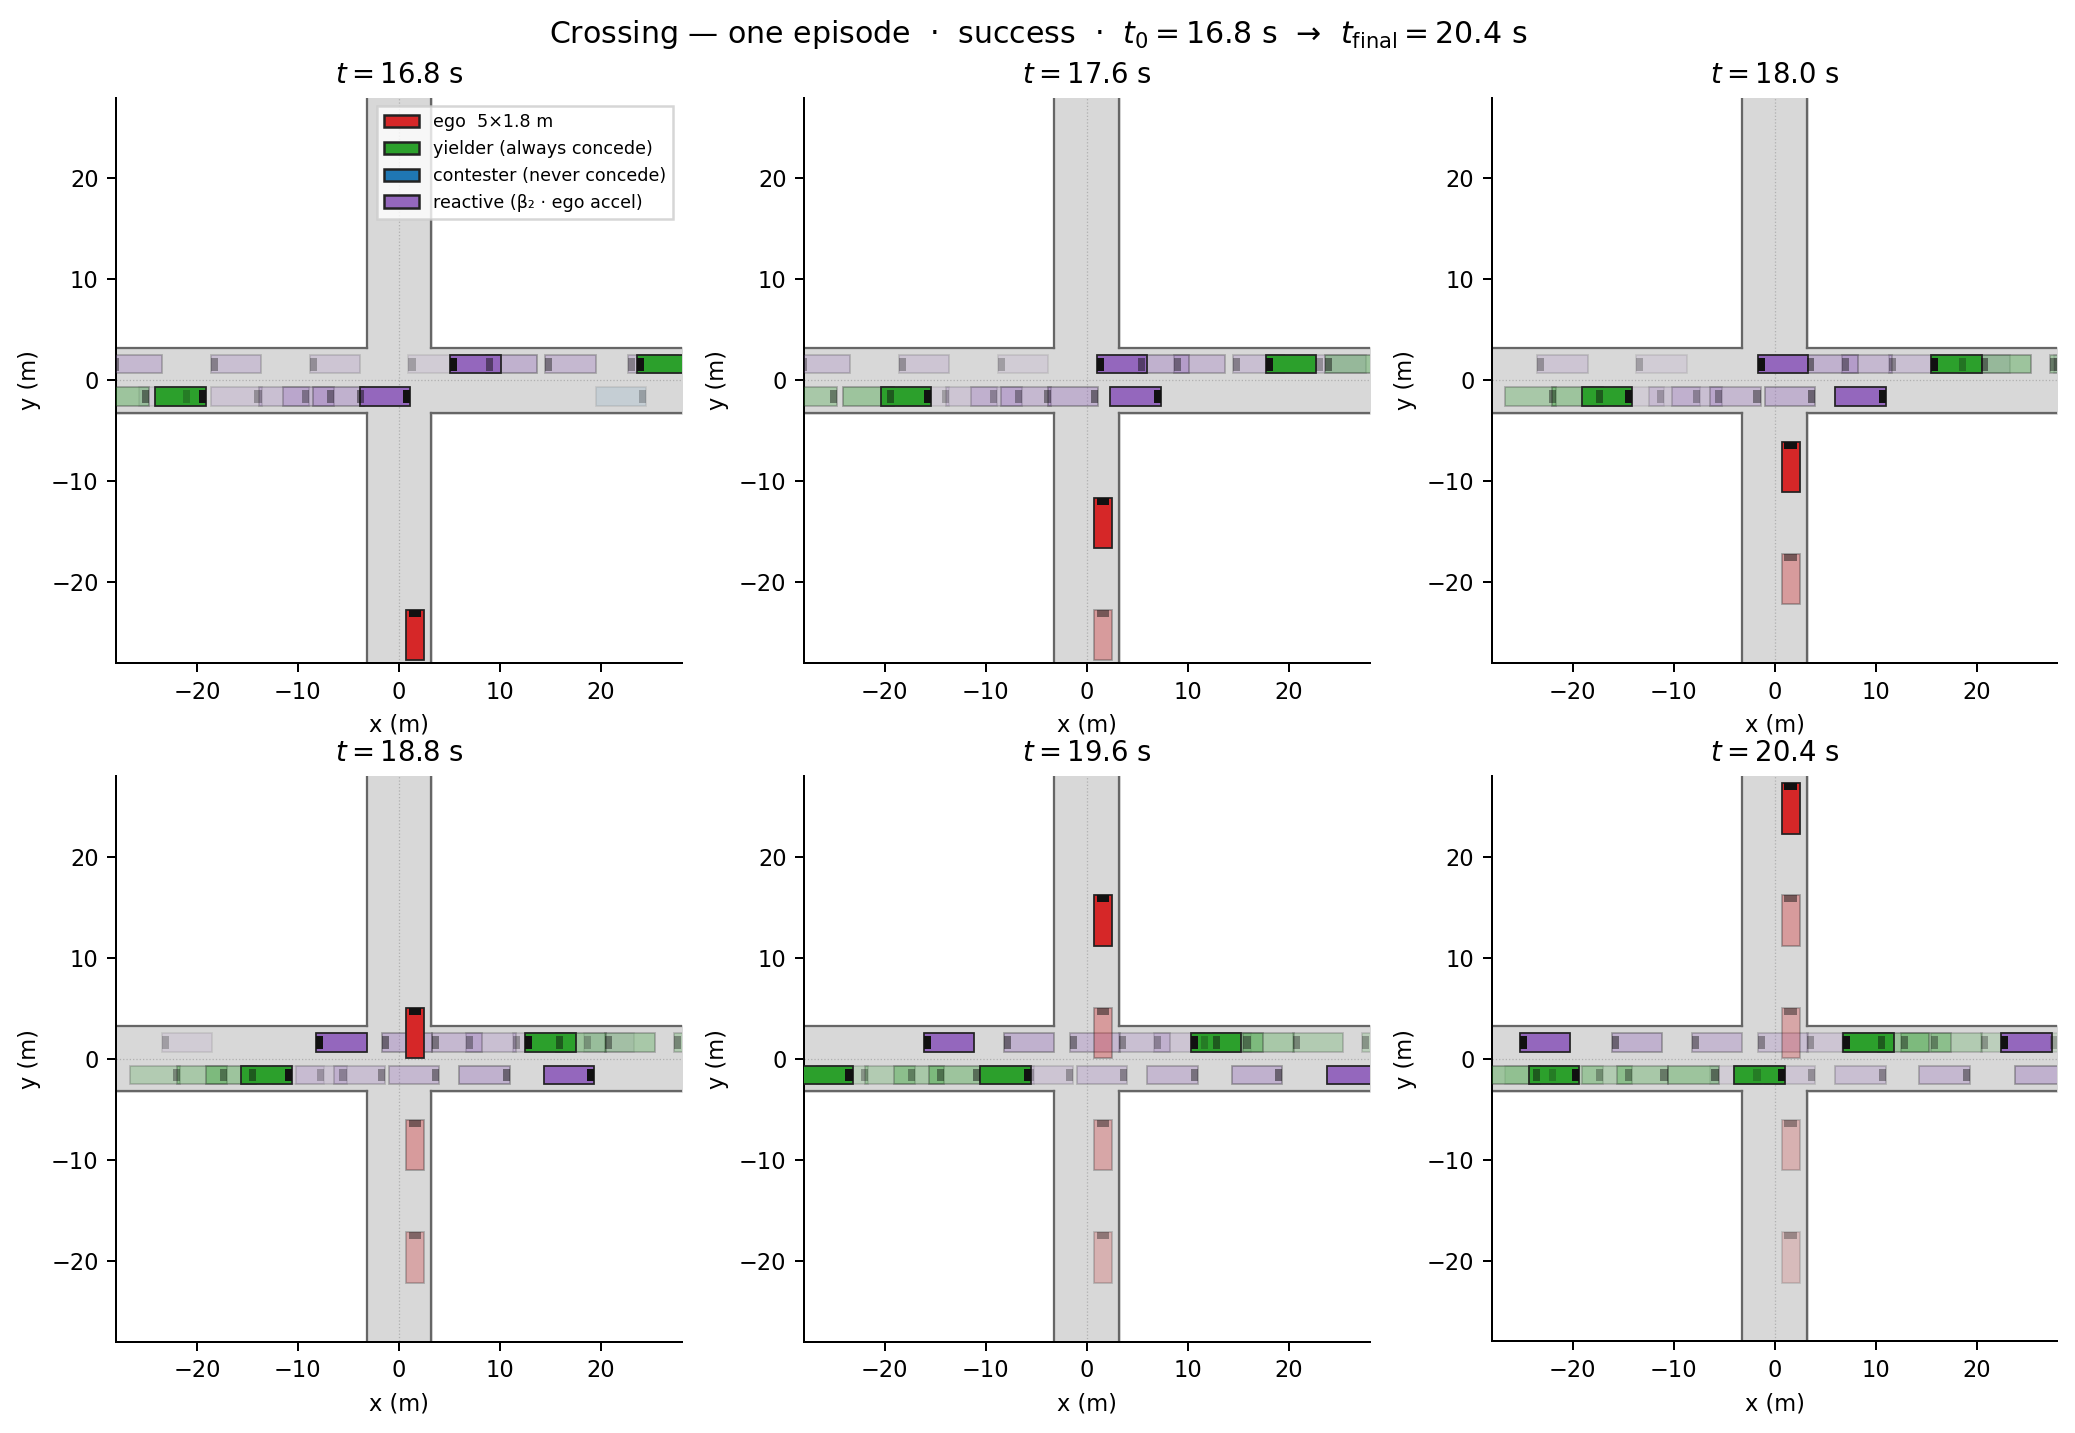
\includegraphics[width=0.92\textwidth]{figures/time_sequence/setup_cross_trajectories.png}
\caption{Crossing running example: one successful episode, six frames from $t_0$ to $t_{\mathrm{final}}$. Vehicles are $5{\times}1.8$\,m. Red: ego; green/blue/purple: yielder / contester / reactive. Ghosted rectangles are recent history. Merge and roundabout sequences follow (Fig.~\ref{fig:setup-scenes-app}).}
\label{fig:setup-cross}
\end{figure*}

\begin{figure*}[!t]
\centering
\subfloat[Merge.]{%
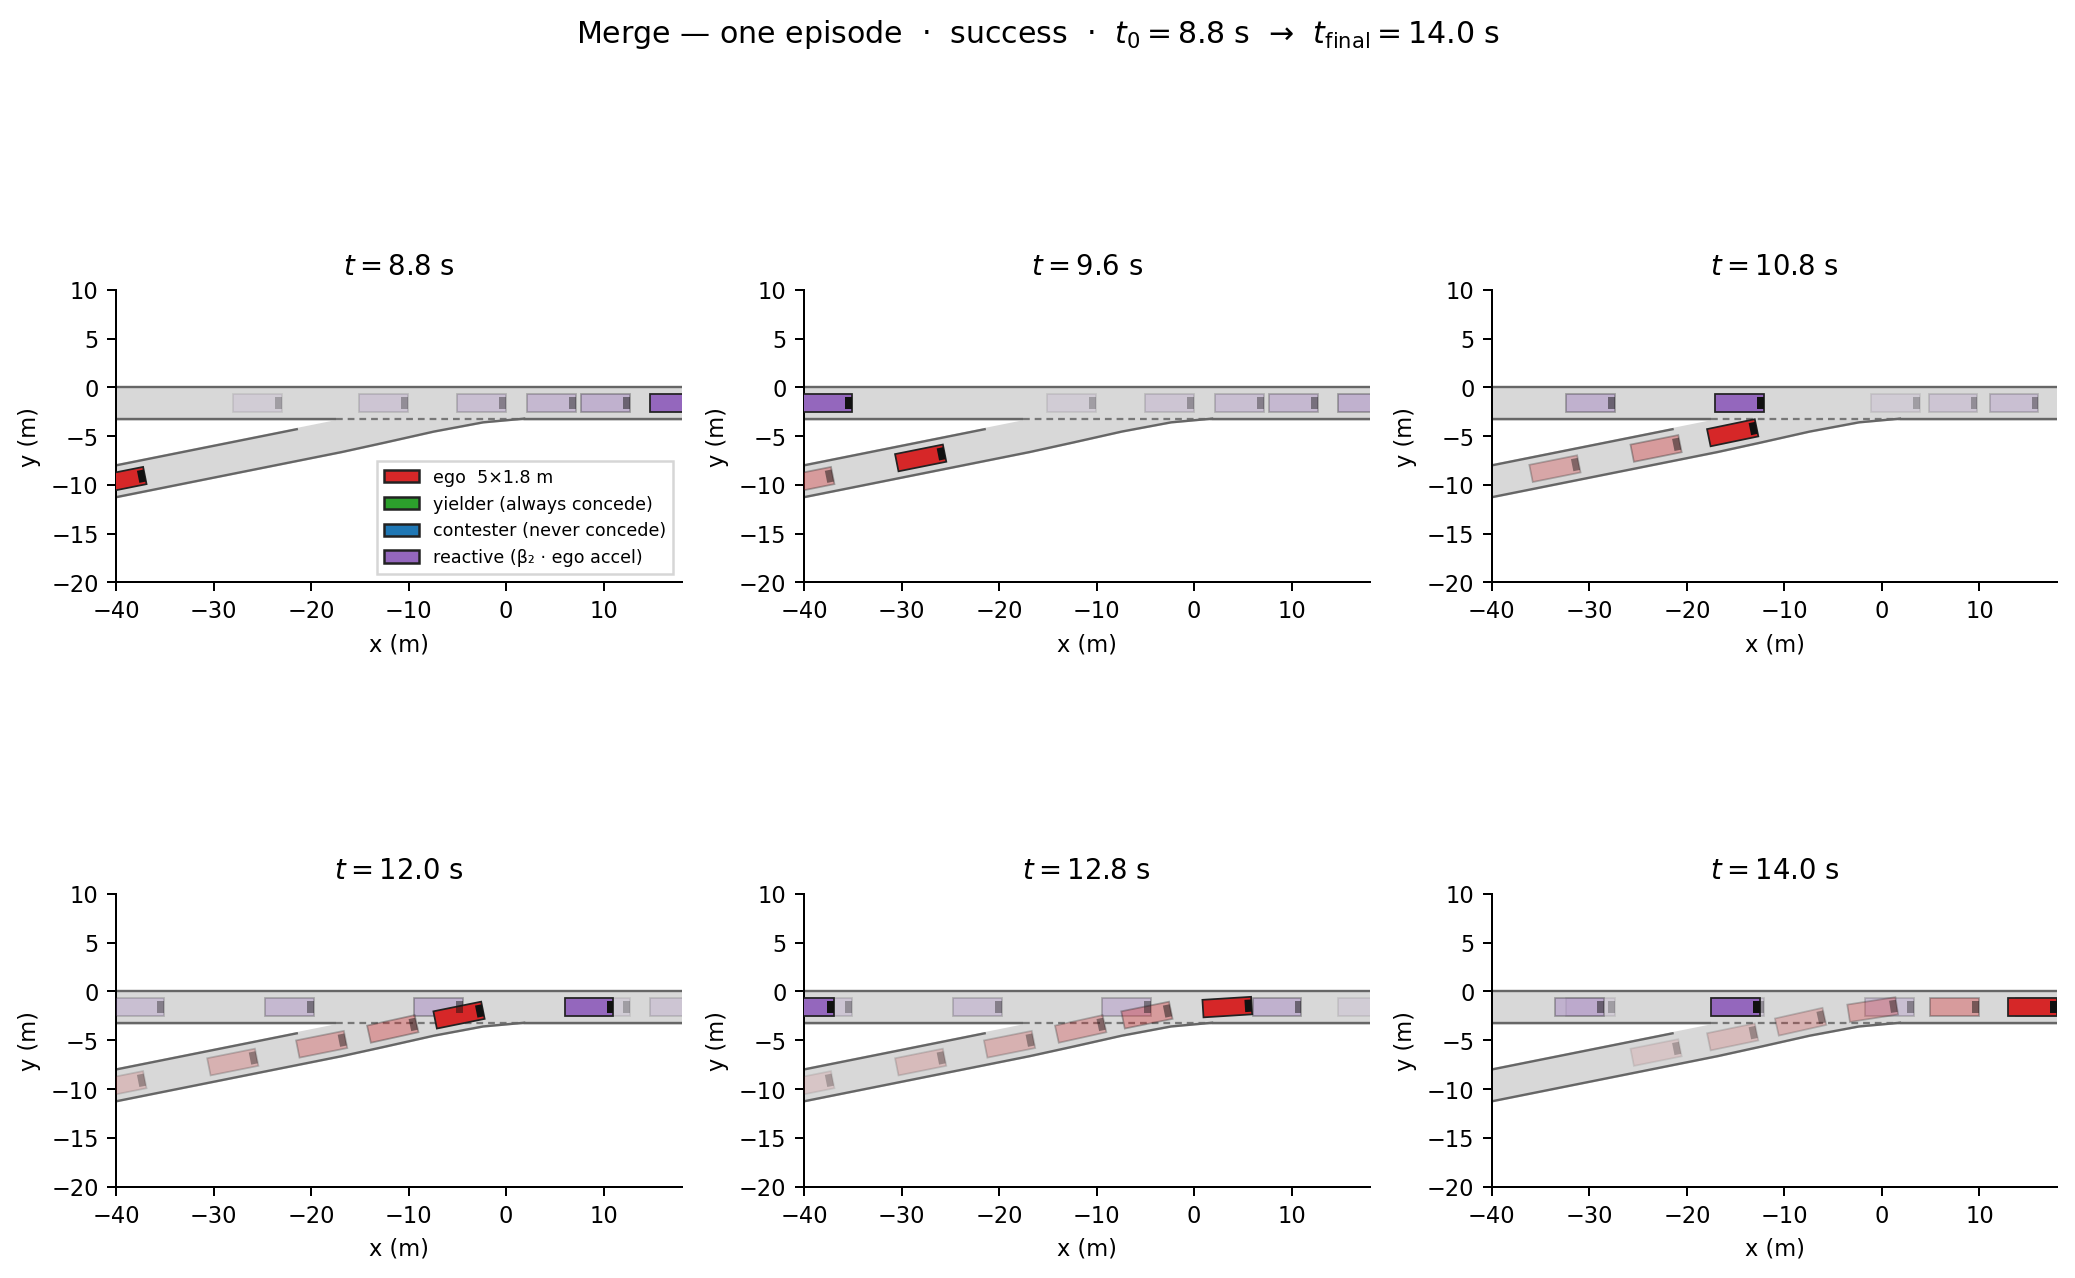
\includegraphics[width=0.92\textwidth]{figures/time_sequence/setup_merge_trajectories.png}%
\label{fig:setup-merge}}\\
\vspace{0.15em}
\subfloat[Roundabout.]{%
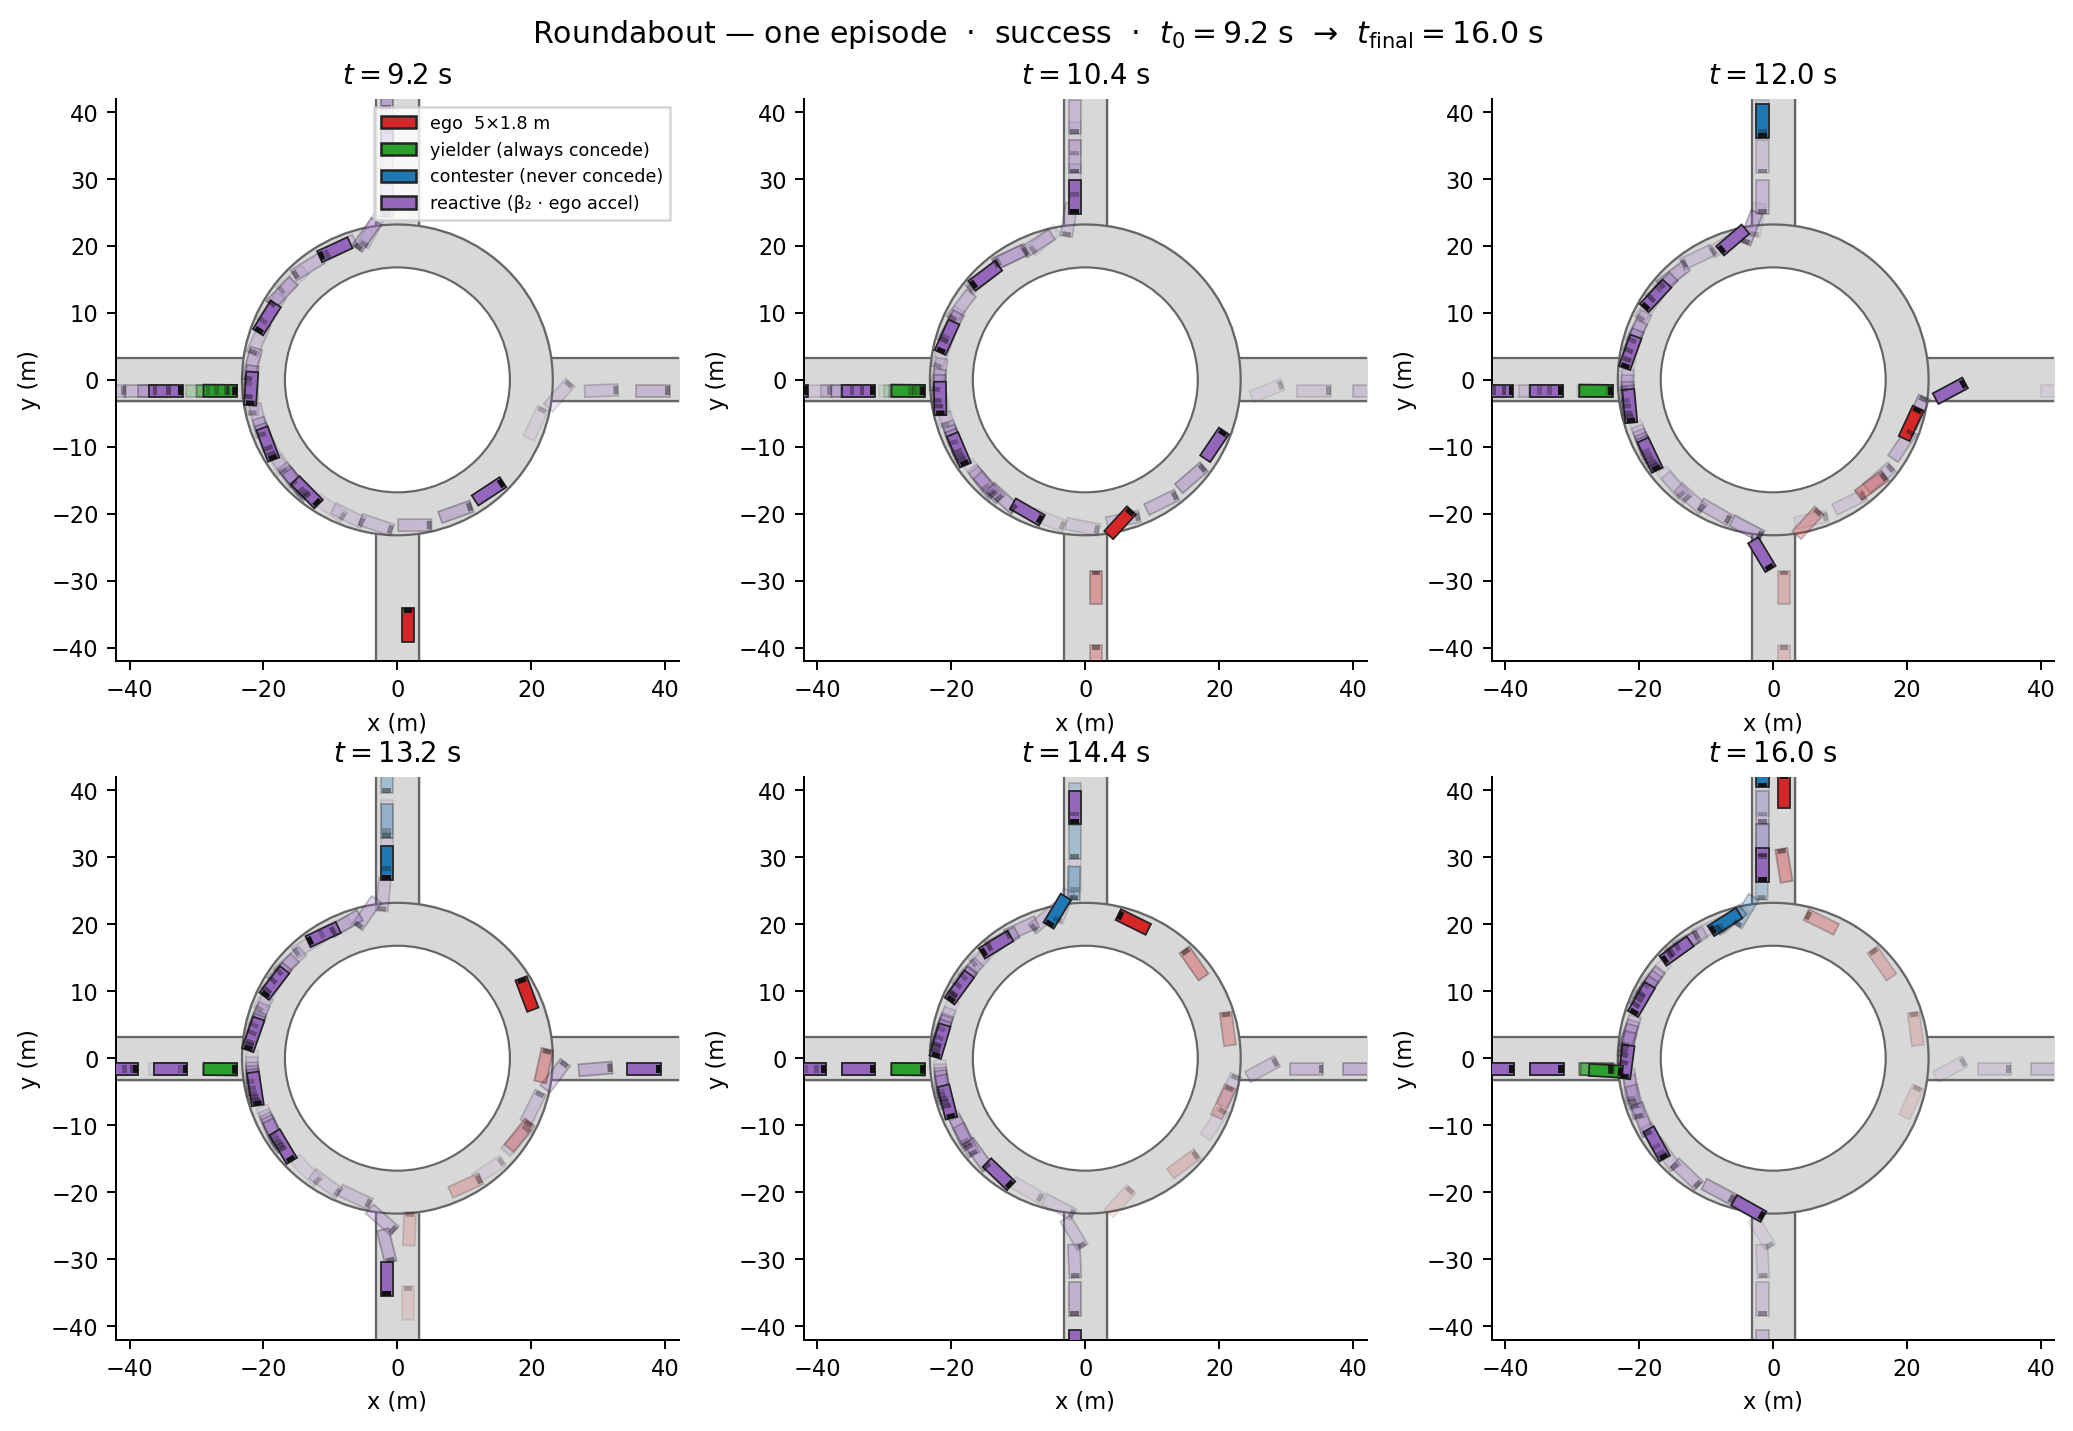
\includegraphics[width=0.92\textwidth]{figures/time_sequence/setup_roundabout.png}%
\label{fig:setup-rbt}}
\caption{One successful episode per map, six frames from $t_0$ to $t_{\mathrm{final}}$, matching Fig.~\ref{fig:setup-cross}. Vehicles are $5{\times}1.8$\,m. Red: ego; green/blue/purple: yielder / contester / reactive.}
\label{fig:setup-scenes-app}
\end{figure*}

\begin{figure*}[!t]
\centering
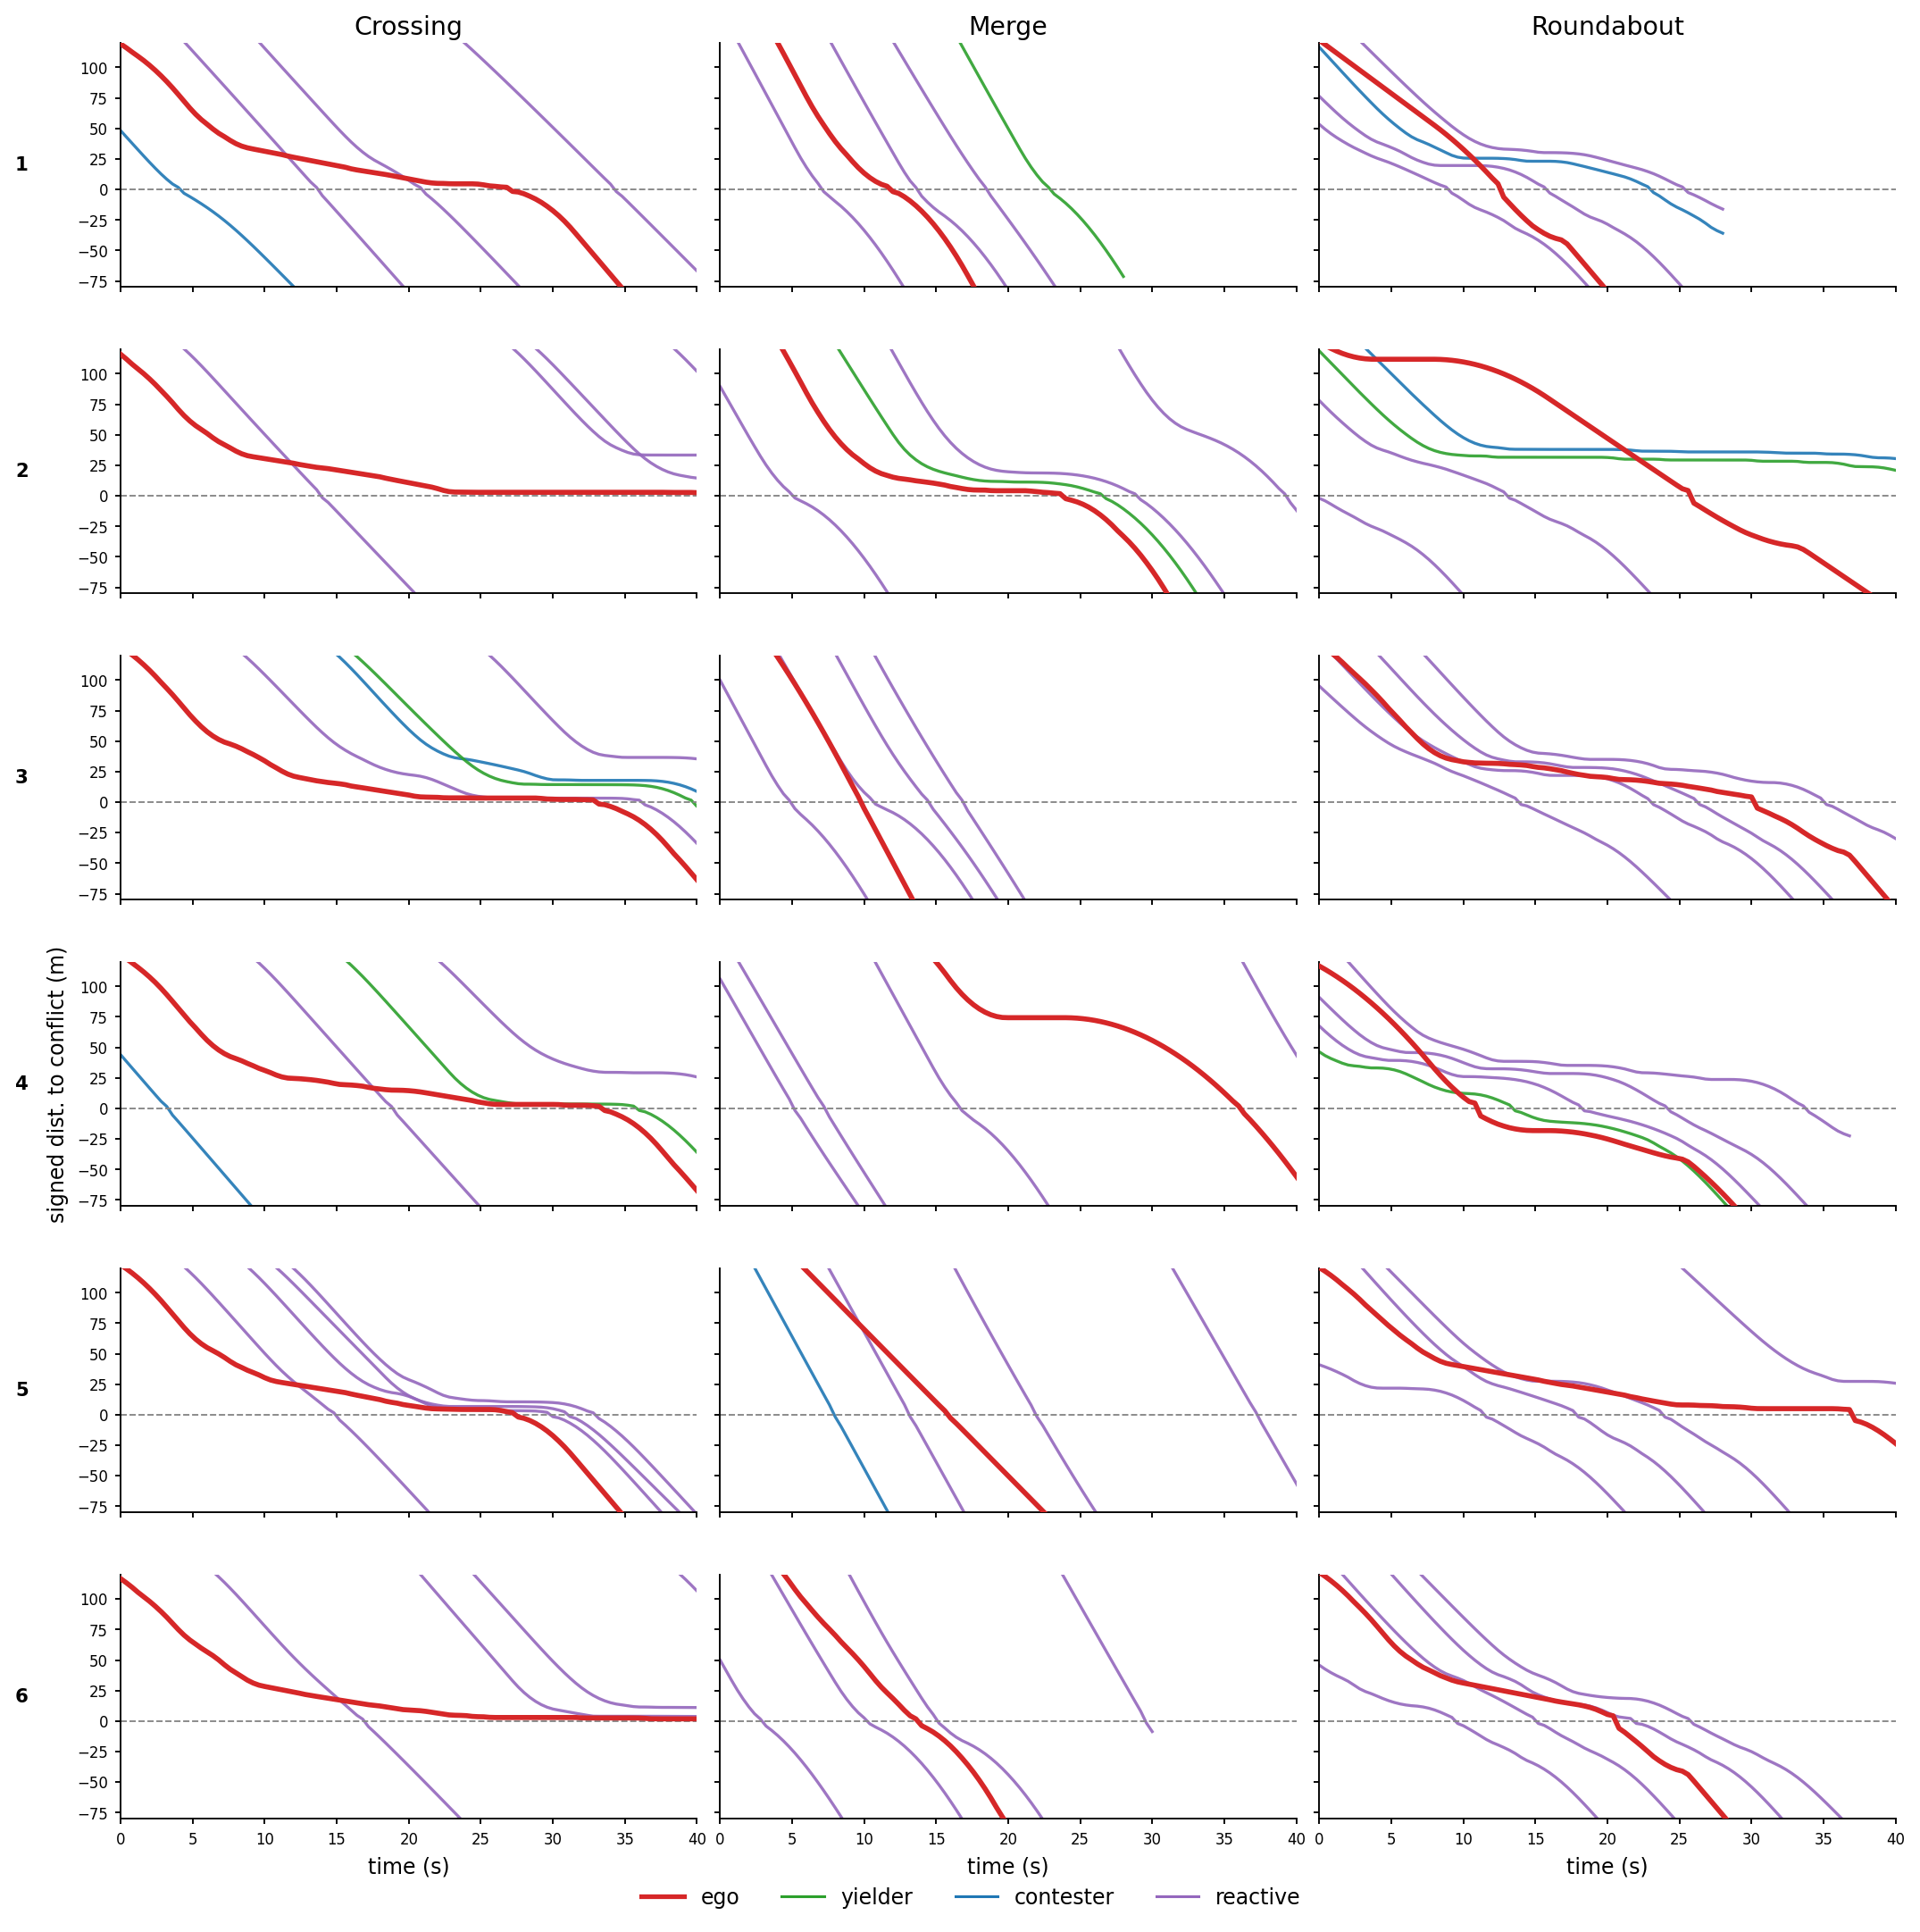
\includegraphics[width=\textwidth]{figures/setup_distance_samples.png}
\caption{Signed distance to the conflict for six successful episodes per map (rows). Red: ego; green/blue/purple: yielder / contester / reactive. $d{=}0$ is the conflict. A plateau just above zero is waiting; a crossing of the dashed line is clearance.}
\label{fig:setup-dt}
\end{figure*}

\subsection{Deciding-neighbour evaluation}

The population matters, and getting it wrong hides the channel. A neighbour's intention responds to the ego's plan only if that neighbour is about to commit. Most vehicles in a scene are not: they are far from the conflict
point, or have already passed it, or already decided. Their behaviour genuinely
does not depend on what the ego does next, and averaging over them is averaging
mostly zeros. Measured over all present neighbours, our model's probe response
spans a total variation of only \tvModelAll{} (still monotone, but flattened
by the zeros). Measured over the
neighbours that actually commit within the plan horizon --- the population the
counterfactual query is about --- the same model spans \tvModelDec{} against a
ground-truth \gtTV{}, and is monotone in the correct direction. We report both,
because the first number is the one an incautious evaluation would produce and it
is misleading. Even on the deciding population the recovered TV
(\tvModelDec{}) is weaker than the simulator (\gtTV{}), and trajectory shifts sit
near the sample spread (\probeSpread{}\,m): yield vs hold moves forecasts by
\probeShiftBrake{}\,m, assert vs hold by \probeShiftAssert{}\,m. Directional
recovery of $q_\phi$ is therefore not evidence that the planner receives a usable
counterfactual trajectory signal.

The same consideration applies to the belief features and is not merely
diagnostic. Pooling per-neighbour intentions by a plain average makes that
component of $\psi_t$ nearly constant across probes, so the policy receives no
usable intention signal; we therefore pool the most dangerous partner (minimum
$\Pr(\yield)$, maximum $\Pr(\contest)$ among neighbours that can reach the
conflict in the query horizon).
This has a corresponding cost in the supervision: the intention head is trained
only on neighbours whose decision falls inside the prediction window, which is
$\labelledFrac{}$ of neighbour slots. Labelling every slot with the episode's
eventual outcome, as would be natural, supervises the head mostly with decisions
that were taken before $t$ or long after $t+F$, and drives it to the marginal.

\subsection{Additional tables}

\begin{figure*}[!t]
\centering
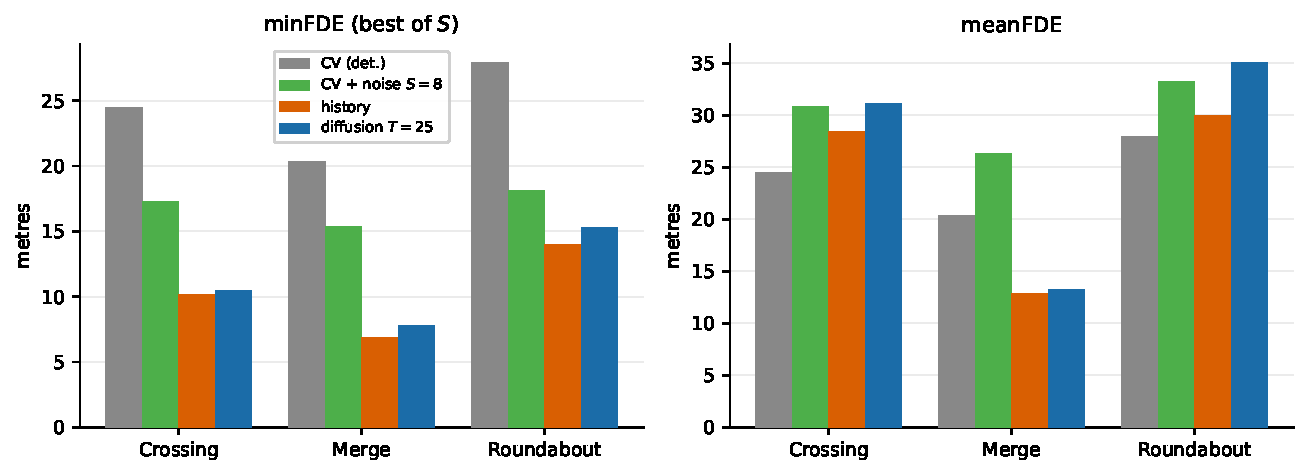
\includegraphics[width=0.92\textwidth]{figures/results_extra/wm_fde.pdf}
\caption{Held-out displacement error on all three maps. minFDE is a best-of-$S$
statistic; meanFDE is the proper comparison to deterministic constant velocity.
History is competitive on minFDE; diffusion meanFDE does not dominate CV on the
crossing.}
\label{fig:wm-fde}
\end{figure*}

\begin{figure*}[!t]
\centering
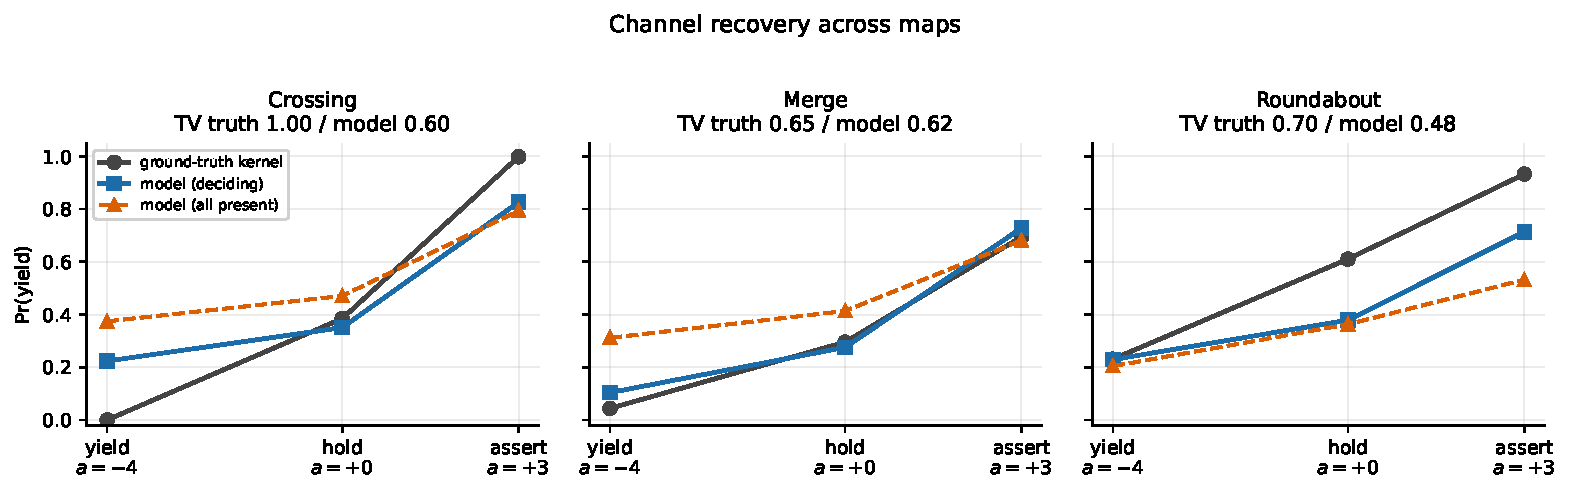
\includegraphics[width=0.96\textwidth]{figures/results_extra/channel_scenes.pdf}
\caption{Same intention-head probe as Fig.~\ref{fig:channel}, on all three maps.
The deciding-neighbour population is the relevant one. Merge recovers almost
all of the kernel TV; the roundabout recovers the direction but not the
magnitude.}
\label{fig:channel-scenes}
\end{figure*}

Table~\ref{tab:sweep} and Fig.~\ref{fig:sweep} vary $S$. $S{=}8$ is the
operating point of Table~\ref{tab:planner} (copied from the main crossing
suite); $S\in\{1,4,16\}$ were retrained for $40$ PPO iterations under the
louder channel. Table~\ref{tab:beta} is the matched $\beta_2{=}0$ versus
$\beta_2{=}4.0$ control (the $\beta_2{=}0$ rows repeat Table~\ref{tab:influence}).
Tables~\ref{tab:shift} and~\ref{tab:hard} are zero-shot evaluations with no
retraining. Table~\ref{tab:baselines} reports rule baselines on the crossing.
Table~\ref{tab:independent} compares a joint residual to an independent
per-neighbour world model on matched seeds.
Table~\ref{tab:cf} and Fig.~\ref{fig:cf-shift} score interventional neighbour
shift against $\mathrm{do}(u)$ replays.
Main closed-loop tables for crossing, merge, and roundabout appear in
Section~\ref{sec:exp:planner}.

\begin{figure*}[!t]
\centering
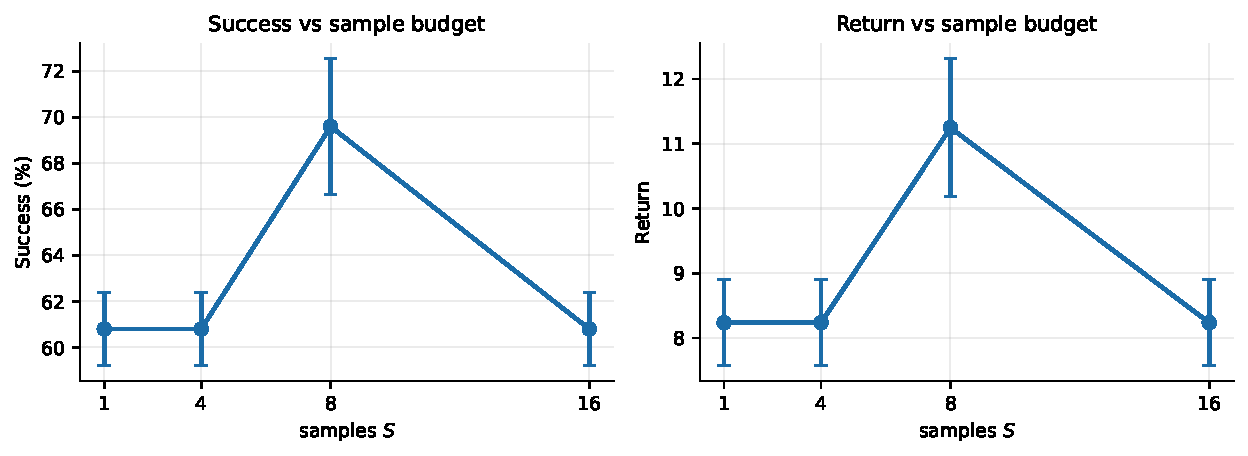
\includegraphics[width=0.88\textwidth]{figures/results_extra/sweep_S.pdf}
\caption{Closed-loop success and return versus belief sample budget $S$ on the
crossing. $S{=}8$ is the main-suite operating point; $S\in\{1,4,16\}$ were
retrained for fewer iterations and do not separate under the risk/clear/intent
belief interface.}
\label{fig:sweep}
\end{figure*}

\begin{table*}[!t]
\caption{Sample budget $S$ for the belief features. Remark~\ref{rem:hoeffding} bounds the $95\%$ resolution of the risk estimate by $\epsilon \approx \sqrt{\ln(40)/(2S)}$, shown for reference. $S{=}8$ is copied from the main crossing suite ($60$ iterations); $S\in\{1,4,16\}$ use $40$ iterations under the louder channel. Mean $\pm$ s.d.\ over $n{=}5$ seeds.}
\label{tab:sweep}
\centering
\begin{tabular}{|c|c|c|c|c|c|}
\hline
$\boldsymbol{S}$ & $\boldsymbol{\epsilon_{95}}$ & \textbf{Success (\%)} & \textbf{Collision (\%)} & \textbf{Timeout (\%)} & \textbf{Return} \\
\hline
$1$ & $1.37$ & 60.80$\pm$1.60 & 39.20$\pm$1.60 & 0.00$\pm$0.00 & 8.24$\pm$0.67 \\ % n=5
\hline
$4$ & $0.69$ & 60.80$\pm$1.60 & 39.20$\pm$1.60 & 0.00$\pm$0.00 & 8.24$\pm$0.67 \\ % n=5
\hline
$8$ & $0.48$ & 69.60$\pm$2.94 & 30.00$\pm$3.35 & 0.40$\pm$0.80 & 11.25$\pm$1.06 \\ % n=5, planner\_cross
\hline
$16$ & $0.34$ & 60.80$\pm$1.60 & 39.20$\pm$1.60 & 0.00$\pm$0.00 & 8.24$\pm$0.67 \\ % n=5
\hline
\end{tabular}
\end{table*}

\begin{table*}[!t]
\caption{Interventional counterfactuals on the unsignalised crossing ($n{=}33$ matched scenes). The same scene $h$ is replayed under several ego plans $\mathrm{do}(u)$ in the simulator. Shift is mean neighbour displacement vs the hold plan. A history-only model cannot move its forecast with $u$.}
\label{tab:cf}
\centering
\begin{tabular}{|l|c|c|c|c|}
\hline
\textbf{Model} & \textbf{minFDE} & \textbf{meanFDE} & \textbf{Pred.\ shift (m)} & \textbf{GT shift (m)} \\
\hline
Diffusion $p(y\mid h,u)$ & 1.97 & 37.01 & 1.14 & 1.03 \\
\hline
History $p(y\mid h)$ & 1.40 & 26.24 & 0.00 & 1.03 \\
\hline
\end{tabular}
\end{table*}

\begin{figure*}[!t]
\centering
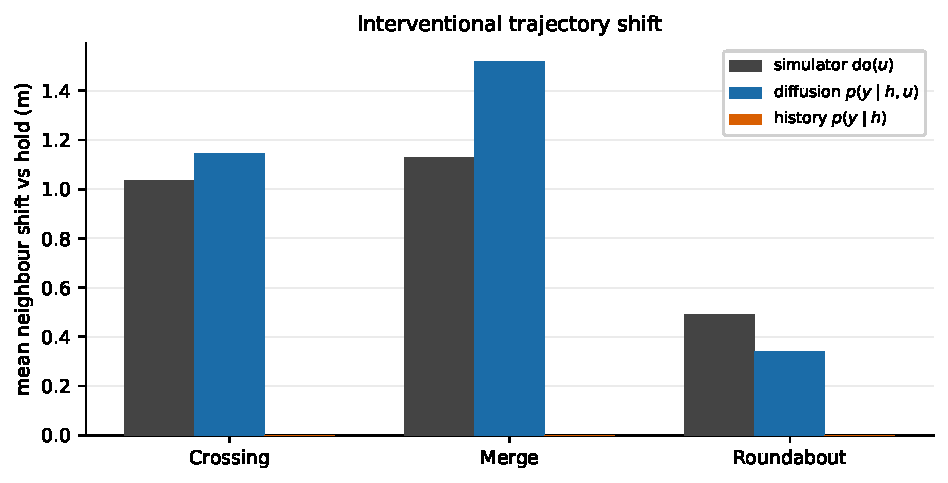
\includegraphics[width=\columnwidth]{figures/results_extra/cf_shift.pdf}
\caption{Interventional neighbour shift versus the hold plan. History cannot
move with $u$ (shift identically zero). Diffusion overshoots the simulator
slightly but has the correct sign on every map.}
\label{fig:cf-shift}
\end{figure*}

\begin{table*}[!t]
\caption{Channel-strength sweep. Same world models (trained with $\beta_2>0$); only the environment kernel changes. \texttt{history} vs \texttt{diffusion} at $\beta_2=0$ is the plan-conditioning ablation with the type-channel removed. On-channel rows use the louder crossing suite ($n{=}10$); off-channel rows use $n{=}5$. Mean $\pm$ s.d.\ over seeds.}
\label{tab:beta}
\centering
\begin{tabular}{|c|l|c|c|c|c|}
\hline
$\boldsymbol{\beta_2}$ & \textbf{Belief} & \textbf{Success (\%)} & \textbf{Collision (\%)} & \textbf{Timeout (\%)} & \textbf{Return} \\
\hline
$0.00$ & \texttt{none} & 62.00$\pm$0.00 & 38.00$\pm$0.00 & 0.00$\pm$0.00 & 9.24$\pm$0.07 \\ % n=5
\hline
$0.00$ & \texttt{history} & 64.40$\pm$2.94 & 35.60$\pm$2.94 & 0.00$\pm$0.00 & 10.00$\pm$1.12 \\ % n=5
\hline
$0.00$ & \texttt{diffusion} & 64.80$\pm$2.04 & 35.20$\pm$2.04 & 0.00$\pm$0.00 & 10.25$\pm$0.94 \\ % n=5
\hline
$4.00$ & \texttt{none} & 61.60$\pm$4.45 & 38.40$\pm$4.45 & 0.00$\pm$0.00 & 8.55$\pm$1.73 \\ % n=10, planner\_cross
\hline
$4.00$ & \texttt{history} & 65.60$\pm$3.20 & 34.40$\pm$3.20 & 0.00$\pm$0.00 & 9.95$\pm$1.09 \\ % n=10, planner\_cross
\hline
$4.00$ & \texttt{diffusion} & 68.00$\pm$3.10 & 31.80$\pm$3.40 & 0.20$\pm$0.60 & 10.82$\pm$1.11 \\ % n=10, planner\_cross
\hline
\end{tabular}
\end{table*}

\begin{table*}[!t]
\caption{Zero-shot shift evaluation (denser traffic / more contested type mix; channel strength held at train-time $\beta_2{=}4.0$). No retraining. Mean $\pm$ s.d.\ over $n{=}10$ seeds.}
\label{tab:shift}
\centering
\begin{tabular}{|l|c|c|c|c|c|c|}
\hline
\textbf{Belief} & \textbf{Success (\%)} & \textbf{Collision (\%)} & \textbf{Timeout (\%)} & \textbf{Return} & \textbf{Crossing steps} & \textbf{Induced brakes} \\
\hline
\texttt{none} (no world model) & 69.60$\pm$4.45 & 30.40$\pm$4.45 & 0.00$\pm$0.00 & 11.94$\pm$2.09 & 59.69$\pm$2.67 & 0.00$\pm$0.00 \\ % n=10
\hline
\texttt{geometry} (ego-plan CV risk) & 67.80$\pm$3.03 & 31.60$\pm$3.56 & 0.60$\pm$1.28 & 10.94$\pm$1.35 & 60.06$\pm$2.93 & 0.00$\pm$0.00 \\ % n=10
\hline
\texttt{kernel} (analytic channel feature) & 66.60$\pm$4.10 & 32.80$\pm$3.60 & 0.60$\pm$0.92 & 10.45$\pm$1.83 & 58.10$\pm$4.34 & 0.00$\pm$0.00 \\ % n=10
\hline
\texttt{history} (plan dropped) & 68.20$\pm$2.27 & 31.40$\pm$1.80 & 0.40$\pm$0.80 & 11.10$\pm$1.19 & 58.84$\pm$3.31 & 0.00$\pm$0.00 \\ % n=10
\hline
\texttt{diffusion} (multi-hypothesis) & 67.00$\pm$2.41 & 32.40$\pm$2.65 & 0.60$\pm$0.92 & 10.51$\pm$1.20 & 60.16$\pm$3.92 & 0.00$\pm$0.00 \\ % n=10
\hline
\end{tabular}
\end{table*}

\begin{table*}[!t]
\caption{Harder traffic mix (denser, more contested types; channel strength held at train-time $\beta_2{=}4.0$). No retraining. Mean $\pm$ s.d.\ over $n{=}10$ seeds.}
\label{tab:hard}
\centering
\begin{tabular}{|l|c|c|c|c|c|c|}
\hline
\textbf{Belief} & \textbf{Success (\%)} & \textbf{Collision (\%)} & \textbf{Timeout (\%)} & \textbf{Return} & \textbf{Crossing steps} & \textbf{Induced brakes} \\
\hline
\texttt{none} (no world model) & 63.60$\pm$1.96 & 36.40$\pm$1.96 & 0.00$\pm$0.00 & 9.33$\pm$0.87 & 59.23$\pm$2.12 & 0.00$\pm$0.00 \\ % n=10
\hline
\texttt{geometry} (ego-plan CV risk) & 60.60$\pm$4.39 & 38.60$\pm$4.00 & 0.80$\pm$0.98 & 7.71$\pm$1.86 & 60.29$\pm$4.01 & 0.00$\pm$0.00 \\ % n=10
\hline
\texttt{kernel} (analytic channel feature) & 62.60$\pm$6.58 & 36.60$\pm$6.87 & 0.80$\pm$1.33 & 8.58$\pm$2.74 & 59.41$\pm$4.71 & 0.00$\pm$0.00 \\ % n=10
\hline
\texttt{history} (plan dropped) & 64.00$\pm$3.10 & 35.00$\pm$3.00 & 1.00$\pm$1.00 & 9.19$\pm$1.44 & 59.06$\pm$3.71 & 0.00$\pm$0.00 \\ % n=10
\hline
\texttt{diffusion} (multi-hypothesis) & 67.00$\pm$5.60 & 32.20$\pm$5.96 & 0.80$\pm$1.33 & 10.30$\pm$2.31 & 61.45$\pm$4.76 & 0.00$\pm$0.00 \\ % n=10
\hline
\end{tabular}
\end{table*}

\begin{table*}[!t]
\caption{Rule-based baselines on the unsignalised crossing (same louder channel and type mix as the PPO arms; $80$ episodes $\times$ $3$ seeds).}
\label{tab:baselines}
\centering
\begin{tabular}{|l|c|c|c|c|}
\hline
\textbf{Policy} & \textbf{Success (\%)} & \textbf{Collision (\%)} & \textbf{Timeout (\%)} & \textbf{Return} \\
\hline
\texttt{gap} (time-gap acceptance) & 83.75 & 16.25 & 0.00 & 10.45 \\
\hline
\texttt{constant} (always-go) & 62.50 & 37.50 & 0.00 & 9.85 \\
\hline
\end{tabular}
\end{table*}

\begin{table*}[!t]
\caption{Independent per-neighbour diffusion world model versus the joint residual on the crossing, mean $\pm$ s.d.\ over matched $n{=}5$ seeds. Independent planners use $40$ PPO iterations; the joint arm is the corresponding main-suite diffusion seeds.}
\label{tab:independent}
\centering
\begin{tabular}{|l|c|c|c|c|c|c|}
\hline
\textbf{Belief} & \textbf{Success (\%)} & \textbf{Collision (\%)} & \textbf{Timeout (\%)} & \textbf{Return} & \textbf{Crossing steps} & \textbf{Induced brakes} \\
\hline
\texttt{diffusion} (joint) & 69.60$\pm$2.94 & 30.00$\pm$3.35 & 0.40$\pm$0.80 & 11.25$\pm$1.06 & 65.78$\pm$5.58 & 0.00$\pm$0.00 \\ % n=5, planner\_cross seeds0-4
\hline
\texttt{independent} (per neighbour) & 62.00$\pm$4.20 & 38.00$\pm$4.20 & 0.00$\pm$0.00 & 8.50$\pm$1.51 & 58.98$\pm$1.63 & 0.00$\pm$0.00 \\ % n=5
\hline
\end{tabular}
\end{table*}

\subsection{Learning curves}

Learning curves deferred from Section~\ref{sec:exp:planner} are collected here. Fig.~\ref{fig:curves} shows PPO return on the crossing under the operating
point (\texttt{commit\_steps}{=}10). Fig.~\ref{fig:curves-scenes} repeats the
same curves on the merge and roundabout. On the merge and the strengthened
crossing, \texttt{diffusion} pulls away from \texttt{geometry}; on the
roundabout the arms stay closer, matching the closed-loop tables in
Section~\ref{sec:exp:planner}.

\begin{figure*}[!t]
\centering
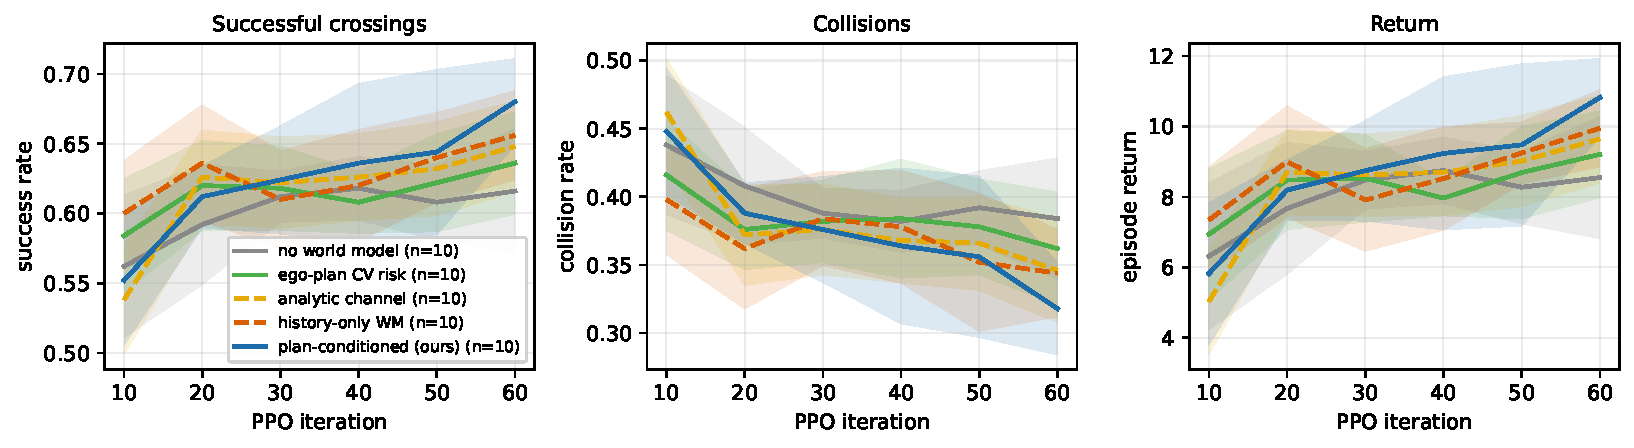
\includegraphics[width=0.92\textwidth]{figures/curves.pdf}
\caption{Learning curves on the crossing (mean $\pm$ s.d.\ over seeds). Under
\texttt{commit\_steps}{=}10 and the louder channel, \texttt{diffusion} leads
\texttt{geometry}; \texttt{history} and \texttt{kernel} sit in between.}
\label{fig:curves}
\end{figure*}

\begin{figure*}[!t]
\centering
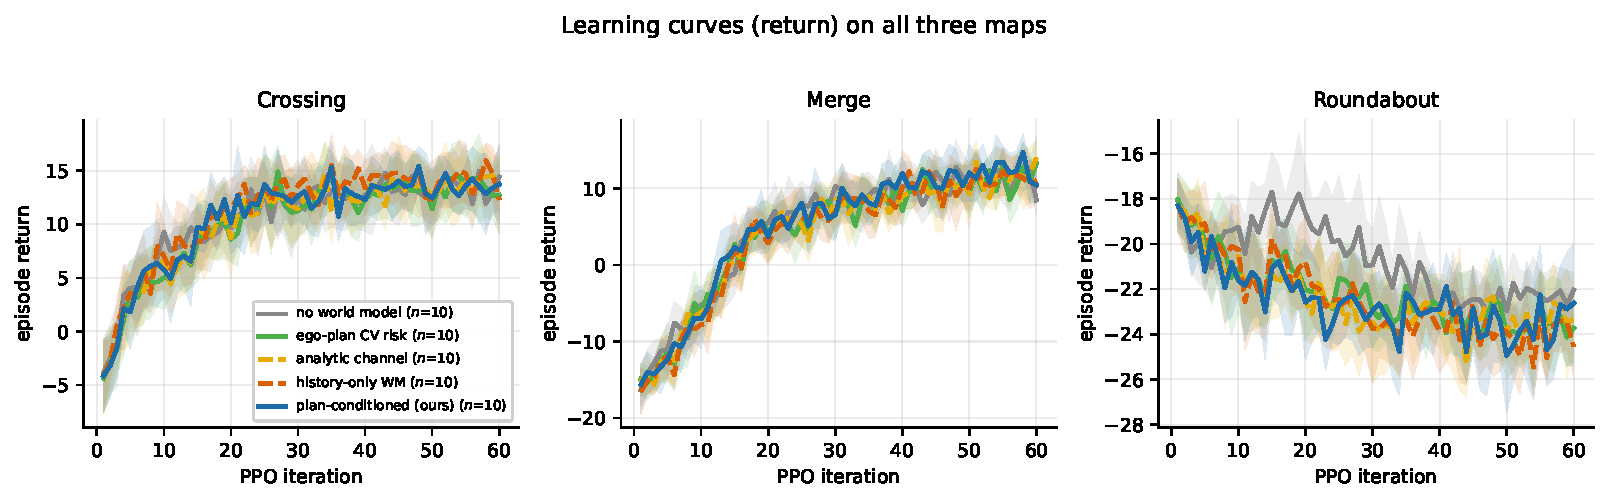
\includegraphics[width=0.96\textwidth]{figures/results_extra/curves_scenes.pdf}
\caption{Return learning curves on all three maps (mean $\pm$ s.d.\ over seeds).
Diffusion pulls away on the merge and the crossing; on the roundabout the arms
stay closer together.}
\label{fig:curves-scenes}
\end{figure*}

\subsection{Compute}

World-model training (120 epochs, batch 256) takes about 20 minutes on one
NVIDIA GPU. Each PPO run is 60 iterations $\times$ 2048 environment steps;
wall-clock is dominated by SUMO and is roughly 6--8 hours per seed
depending on the belief encoder. The default suite targets $10$ seeds $\times$ $5$ arms $\times$ $3$ scenes.
Optional ablations (matched $\beta_2{=}0$, $S$-sweep, independent WM, harder mix /
shift, rule baselines) use the same crossing operating point. All experiments
were run on a local 4-GPU workstation.
Preliminary failed runs (skewed action set, missing timeout penalty) are not
included in the reported seed counts.

\section{Reward Design and Failure Modes}
\label{app:reward}

Two terms deserve comment. The social term is what separates negotiating from bullying: forcing right of way is otherwise free, and an unpenalised agent converges to it. Crucially, a braking event is attributed to the ego only when the ego is near the conflict point \emph{and} the braking vehicle is not simply following a close leader; without that test the statistic is dominated by ordinary queueing and measures traffic density rather than ego behaviour. The liveness term is equally load-bearing for a less interesting reason. Under Eq.~\eqref{eq:reward} without $w_{\text{to}}$, creeping at
$v^\star = w_\tau v_{\max}/w_p \approx 4.2$\,m/s exactly cancels the time penalty, making ``never cross'' a stable local optimum that dominates any exploratory attempt to cross; in preliminary runs every method collapsed onto it. We report this because it is a property of the reward, not of any method, and it would silently invalidate a comparison between methods.

\section{Identification discussion}
\label{app:identification}

This is the step at which conditional-prediction-as-counterfactual claims
usually fail, so we state it explicitly. Suppose the data are generated by a
reactive controller $u = \pi_b(h)$. Then $u$ carries no variation given $h$,
$p(y \mid h, u) = p(y \mid h)$, and evaluating the model at a plan the
controller would not have chosen is extrapolation, not intervention. Worse, if
the controller has episode-level parameters (aggressiveness, accepted gap) that
also influence $y$, those parameters are unobserved confounders and the learned
conditional is biased for the interventional quantity $p(y \mid h, \mathrm{do}(u))$.

We break both problems at the source, in the behaviour policy rather than in the
estimator. Episodes are a mixture: $\approx 8\%$ constant-speed,
$\approx 20\%$ constant acceleration drawn from the discrete action set
$\mathcal{A}=\{-4,-2,0,1,2,3\}$, $\approx 20\%$ piecewise open-loop $F$-step
plans (identifying $\mathrm{do}(u_{1:F})$, not only one-step $u_t$), and
$\approx 52\%$ gap-acceptance with per-action
$\epsilon\sim\mathcal{U}(0.15,0.45)$ drawn per episode. The random and
open-loop components are exogenous by construction, so conditioning on $(h,u)$
identifies $p(y \mid h, \mathrm{do}(u))$ on the support of that mixture --- not
off it. Matched-branch (\texttt{--paired}) collection additionally forks the
same history under several constant-acceleration probes so counterfactual
$\Delta$-losses can supervise response differences. The planner's default
probes $\mathcal{U}=\{-4,0,+3\}$ are constant-acceleration roll-outs of
on-support actions (yield / hold / assert).
Section~\ref{sec:exp:channel} checks that the probe response has the kernel's
\emph{sign}; that is directional recovery, not identification of $\rho$.

\section{Belief-feature construction details}
\label{app:Belief}

Assert-minus-yield contrasts on risk, margin, spread, intention and $\Delta$ bring the vector to $38$ scalars. Relevance pooling is a softmax over predicted closest approach, not identification of ``deciding'' vehicles and that label is evaluation-only.

A \texttt{geometry} ablation replaces the learned world model by constant-velocity neighbour roll-outs against the same probe ego plans, so conflict risk is pure engineered geometry and $\Delta\equiv 0$. A \texttt{kernel} arm uses that same geometry and fills the intention slots from logistic-regression coefficients fitted offline on the world-model dataset (priority margin and plan-acceleration EMA), matching the functional form of the simulator channel without reading $\beta$ or latent types from the live environment. It is a fair engineered baseline for what an accurate channel feature adds over \texttt{geometry}; it is \emph{not} an exact matched-branch oracle. Exact branch evaluation is reported separately when available.

\end{document}
